\chapter{FOSS projects as Cohesive Small Worlds}

As discussed in chapter \ref{collaborative_communities}, we named ``collaborative small world'' the network model that we propose in order to theoretically understand the structural dimension oc cooperation of FOSS projects. We focus here on the empirical analysis of the network structure of two mature and well stablished FOSS projects: the CPython reference implementation of the Python programming language and the Debian Operating System.

These two projects, as outlined in the previous chapter, are quite different despite being both successful FOSS projects. The Debian project has approximately ten times more participants than Python. Debian, being a complete Operating system, has many parts which are only lightly related between them becuse it contains programs that do very different tasks (eg the developers working on packaging software for music editing do not need to pay close attention to what devian developers focused on packaging word processors do). On the other hand, the Python programming language is a much more integrated software projects, and thus developers working on different parts of the language implementation have to play attention, and work very closely, with other developers.

This has a strong impact in the structure of the patterns of relations that emerge between developers in the two projects. The analysis presented here has two parts: first we will compute the small world metrics for the two projects, as described in chapter \ref{collaborative_communities}, and then we will compute the structural cohesion metrics as described in the chapter \ref{structural_cohesion}.

Both kinds of analysis have in common the use of null models in order to assess that the metrics observed in the actual networks are significantly different to the patterns of relations that we might expect if the relation between developers and packages (or developers and files in the case of Python) were produced uniformly at random.

The null model that we use in our analysis is the configuration model (cite properly) in which we preserve the number of developers and packages or files observed in empirical networks along with their degree distributions, that is the null model contains the same number of nodes, edges, and node degrees but the connections between nodes are assigned uniformly at random.

\section{Small World Metrics}

In the first place we compute small world metrics for python networks. The results are shown in table \ref{swi_python}.

\begin{table}[H]
\begin{center}
\begin{small}
\begin{tabular}{|c|c|c|c|c|c|c|c|c|c|}
\hline
Years&Nodes&Developers&Files&Edges&CC&random CC&APL&random APL&SWI ($Q$)\\
\hline
1999&1,146&9&1,137&1,236&0.102&0.039&3.1&3.5&3.0\\
2000&2,172&31&2,141&3,720&0.214&0.135&3.3&3.5&1.7\\
2001&2,511&33&2,478&4,507&0.205&0.129&3.4&3.6&1.7\\
2002&2,317&38&2,279&4,502&0.204&0.129&3.6&3.6&1.6\\
2003&1,805&42&1,763&3,192&0.153&0.112&3.5&3.6&1.4\\
2004&1,850&49&1,801&3,163&0.113&0.093&3.4&3.6&1.3\\
2005&1,007&44&963&1,759&0.129&0.079&3.7&3.7&1.7\\
2006&2,632&52&2,580&6,794&0.235&0.156&2.8&3.2&1.7\\
2007&3,359&51&3,308&7,790&0.223&0.177&2.9&3.3&1.4\\
2008&2,951&59&2,892&7,833&0.231&0.175&3.0&3.3&1.5\\
2009&2,219&58&2,161&4,708&0.228&0.142&3.1&3.4&1.7\\
2010&2,930&63&2,867&6,504&0.175&0.128&3.4&3.5&1.4\\
2011&2,174&63&2,111&4,459&0.145&0.114&3.5&3.6&1.3\\
2012&2,444&65&2,379&4,843&0.124&0.087&3.7&3.8&1.4\\
2013&2,285&63&2,222&4,743&0.147&0.099&3.6&3.7&1.5\\
2014&2,134&62&2,072&4,149&0.138&0.095&3.6&3.7&1.5\\
\hline
\end{tabular}
\caption{Small world metrics for python networks.}
\label{swi_python}
\end{small}
\end{center}
\end{table}



For the Debian project, the results for the small world metrics are presented in table \ref{swi_debian}.

\begin{table}
\begin{center}
\begin{tabular}{|c|c|c|c|c|c|c|c|c|c|}
\hline
Years&Nodes&Developers&Packages&Edges&CC&random CC&APL&random APL&SWI ($Q$)\\
\hline
1999&3258&391&2867&3250&0.127&0.002&9.4&8.8&54.4\\
2000&3590&521&3069&3493&0.136&0.002&9.5&8.9&80.4\\
2001&5921&755&5166&6158&0.050&0.001&8.4&7.9&31.9\\
2002&6839&840&5999&7109&0.079&0.001&9.2&8.0&48.3\\
2003&7244&882&6362&7764&0.102&0.002&9.0&7.7&56.9\\
2004&7971&982&6989&9390&0.155&0.002&8.0&6.6&52.3\\
2005&8317&1037&7280&10242&0.169&0.003&7.5&6.2&44.1\\
2006&9564&1127&8437&12863&0.173&0.005&6.7&5.6&31.7\\
2007&9434&1145&8289&12736&0.144&0.004&6.8&5.6&26.7\\
2008&10605&1212&9393&14226&0.188&0.004&7.1&5.6&33.1\\
2009&11284&1293&9991&15538&0.229&0.006&7.0&5.4&30.8\\
2010&10447&1319&9128&13702&0.282&0.005&7.7&5.6&40.2\\
2011&12265&1333&10932&15862&0.141&0.005&7.5&5.5&21.3\\
2012&8408&1055&7353&9528&0.162&0.003&9.5&6.2&32.9\\
\hline
\end{tabular}
\caption{Small world metrics for debian networks.}
\label{swi_debian}
\end{center}
\end{table}




\section{Structural Cohesion Metrics}

\begin{table}[H]
\begin{center}
\begin{tabular}{|c|c|c|c|c|c|c|c|}
\hline
Years&Nodes&GC&Random GC&GBC&Random GBC&maximum $k$&Random max $k$\\
\hline
1999&1146&66.0\%&100.0\%&6.7\%&6.5\%&3 (1.0\%)&2 (6.5\%)\\
2000&2172&96.5\%&100.0\%&33.4\%&31.4\%&8 (1.2\%)&5 (3.1\%)\\
2001&2511&97.3\%&99.8\%&34.1\%&33.0\%&9 (1.2\%)&6 (2.4\%)\\
2002&2317&100.0\%&99.8\%&38.1\%&36.9\%&9 (2.6\%)&7 (1.9\%)\\
2003&1805&100.0\%&99.2\%&34.8\%&33.1\%&7 (3.3\%)&6 (2.4\%)\\
2004&1850&99.8\%&100.0\%&39.7\%&37.1\%&7 (1.8\%)&5 (2.5\%)\\
2005&1007&99.8\%&100.0\%&45.7\%&44.2\%&5 (5.8\%)&4 (7.6\%)\\
2006&2632&100.0\%&100.0\%&74.2\%&69.8\%&9 (1.5\%)&6 (3.9\%)\\
2007&3359&100.0\%&100.0\%&58.6\%&55.2\%&9 (2.0\%)&6 (2.2\%)\\
2008&2951&100.0\%&99.9\%&64.5\%&61.7\%&10 (2.2\%)&7 (2.5\%)\\
2009&2219&100.0\%&99.9\%&51.0\%&48.5\%&7 (2.8\%)&5 (5.6\%)\\
2010&2930&100.0\%&99.9\%&48.7\%&47.0\%&9 (2.7\%)&7 (2.4\%)\\
2011&2174&100.0\%&99.8\%&47.7\%&45.9\%&8 (2.9\%)&7 (1.7\%)\\
2012&2444&99.8\%&99.8\%&41.1\%&40.3\%&8 (3.4\%)&7 (3.4\%)\\
2013&2285&99.9\%&99.9\%&51.6\%&49.8\%&7 (4.2\%)&6 (4.0\%)\\
2014&2134&100.0\%&99.8\%&44.6\%&43.4\%&7 (2.6\%)&6 (3.1\%)\\
\hline
\end{tabular}
\caption{Structural Cohesion metrics for python networks.}
\label{str_cohesion_python}
\end{center}
\end{table}



\begin{figure}[p]
%\centering
\subfloat[Actual Python network 2000]{
\label{fig:s3d_actual_python_2000}
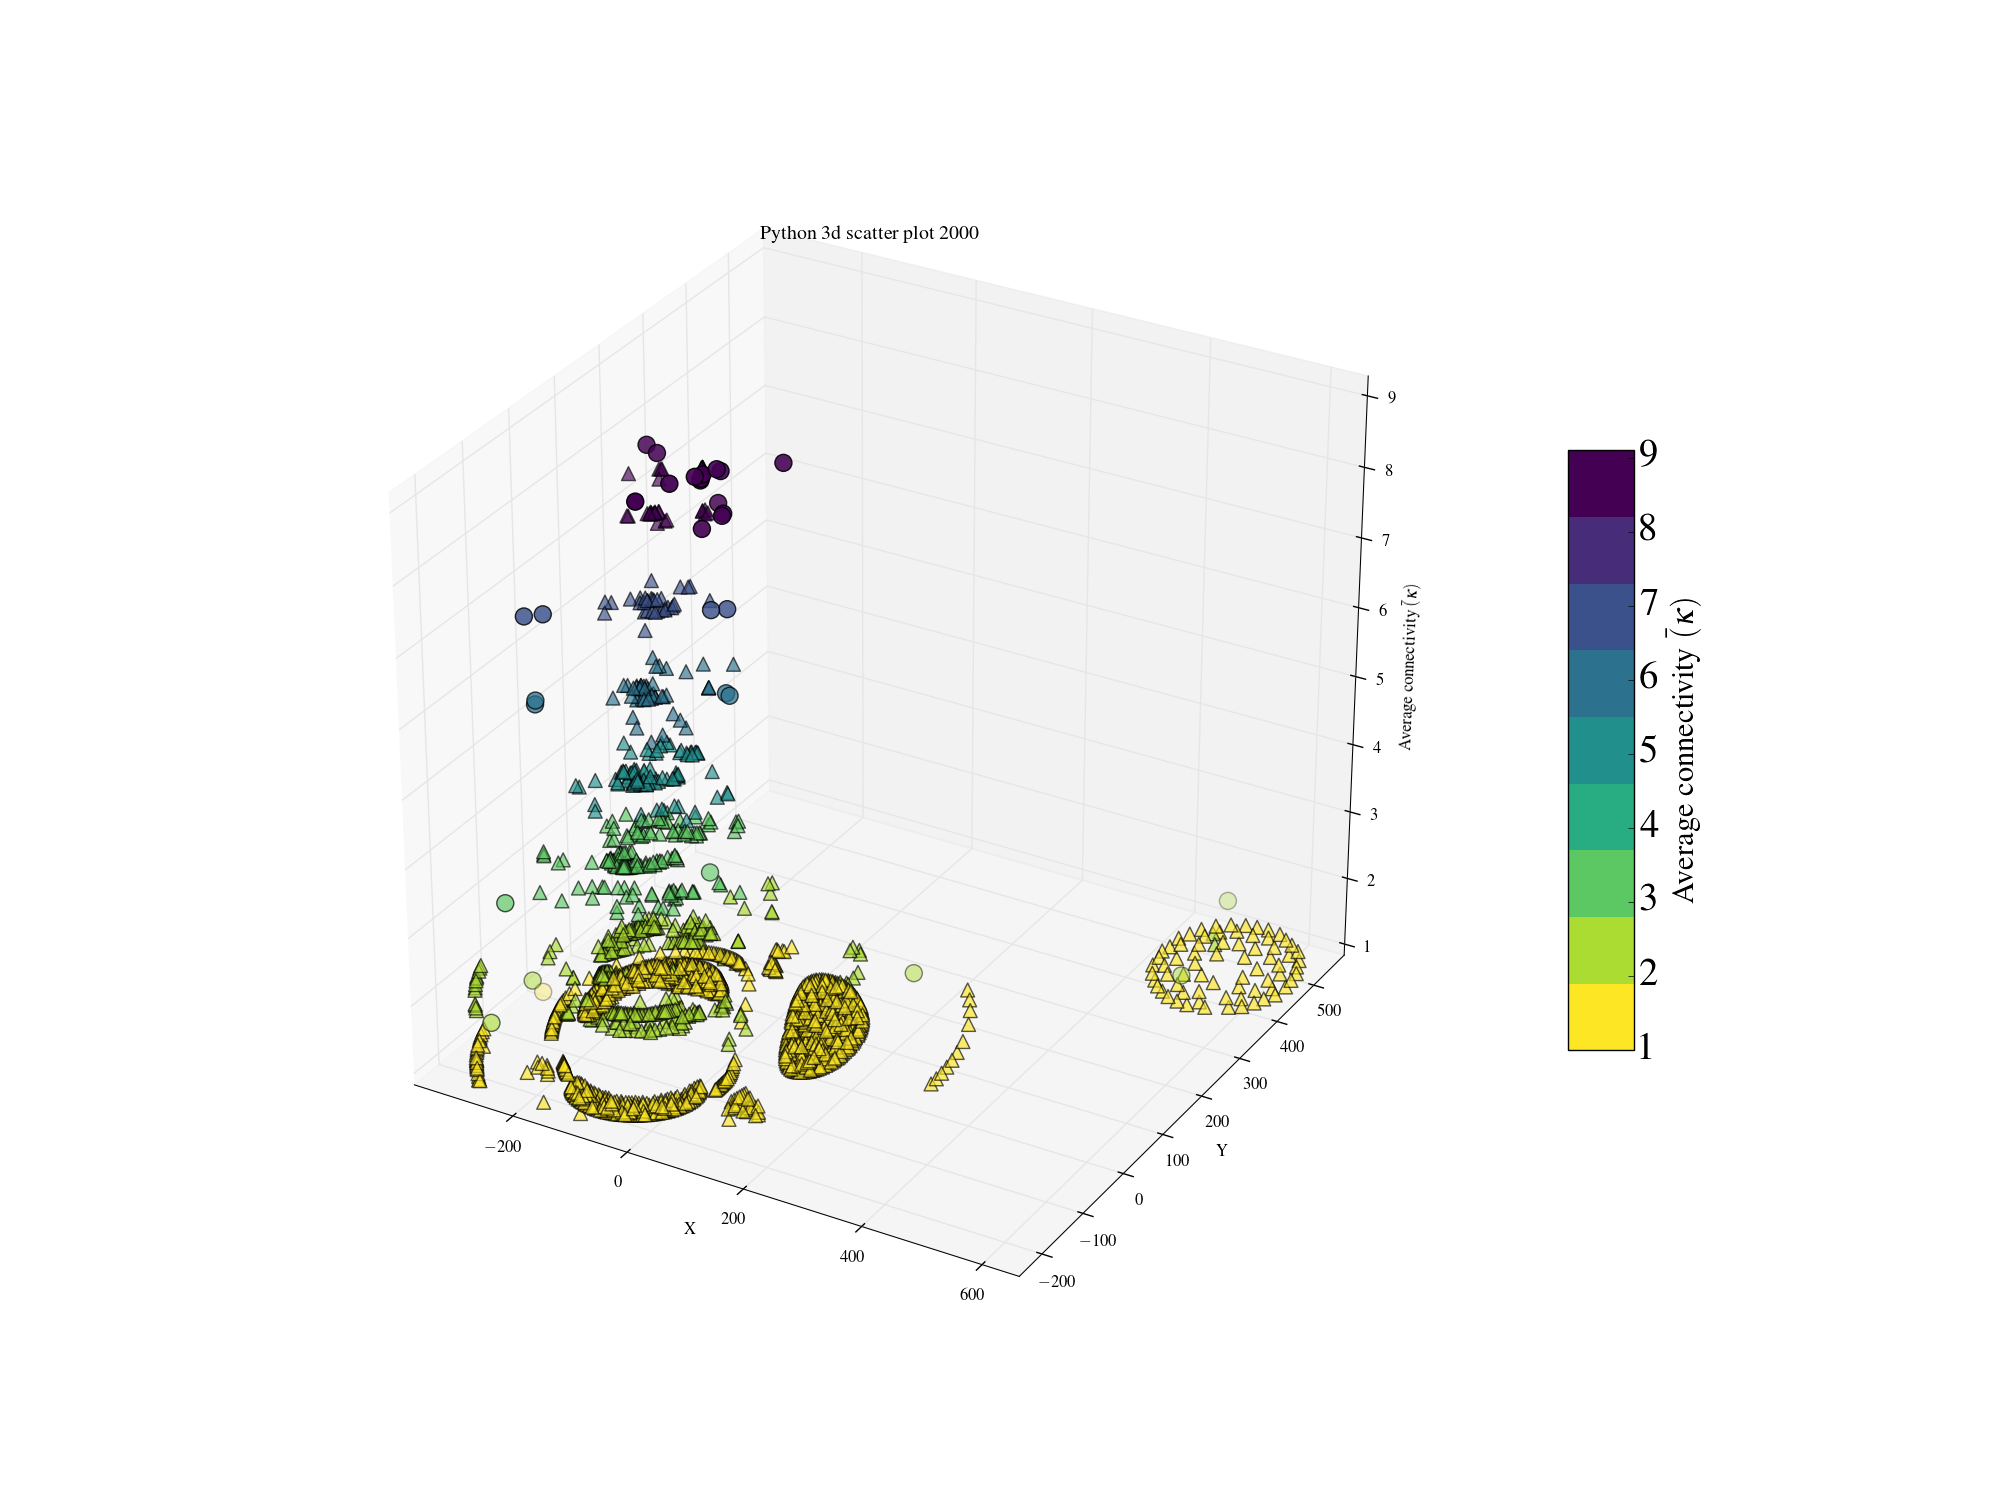
\includegraphics[scale=0.23]{figures/3d_scatter_python_2000}
}
\hspace{.01in}
\subfloat[Null model Python network 2000]{
\label{fig:s3d_null_python_2000}
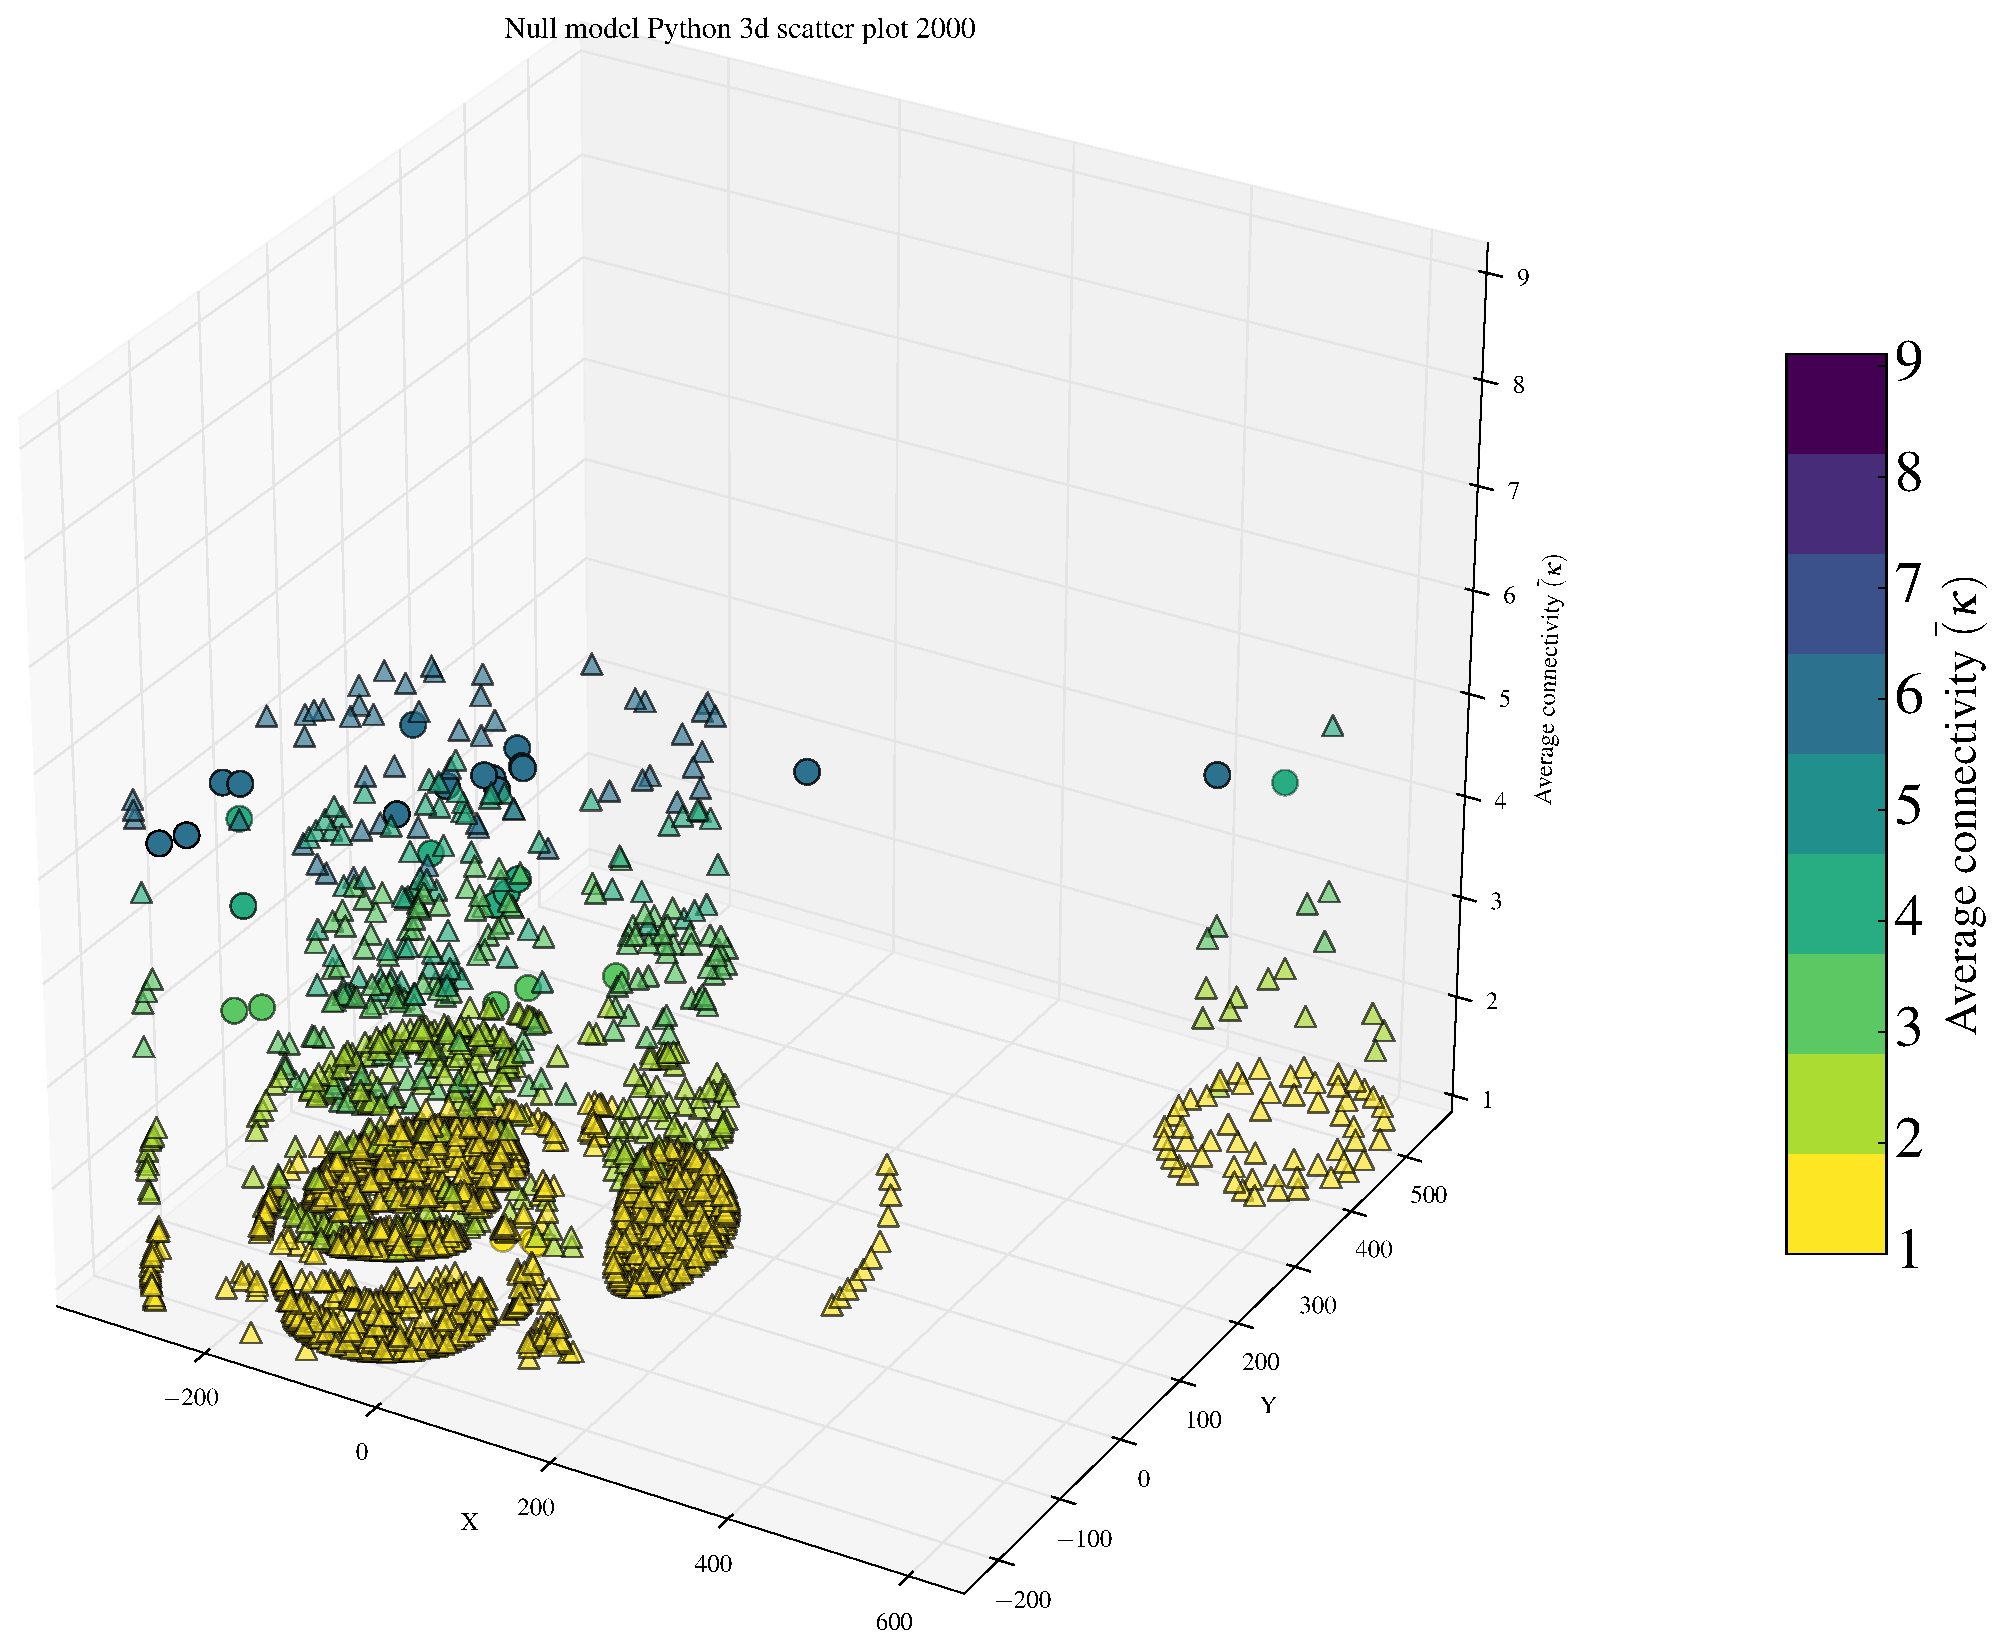
\includegraphics[scale=0.23]{figures/3d_scatter_python_2000_null}
}

\subfloat[Actual Python network 2004]{
\label{fig:s3d_actual_python_2004}
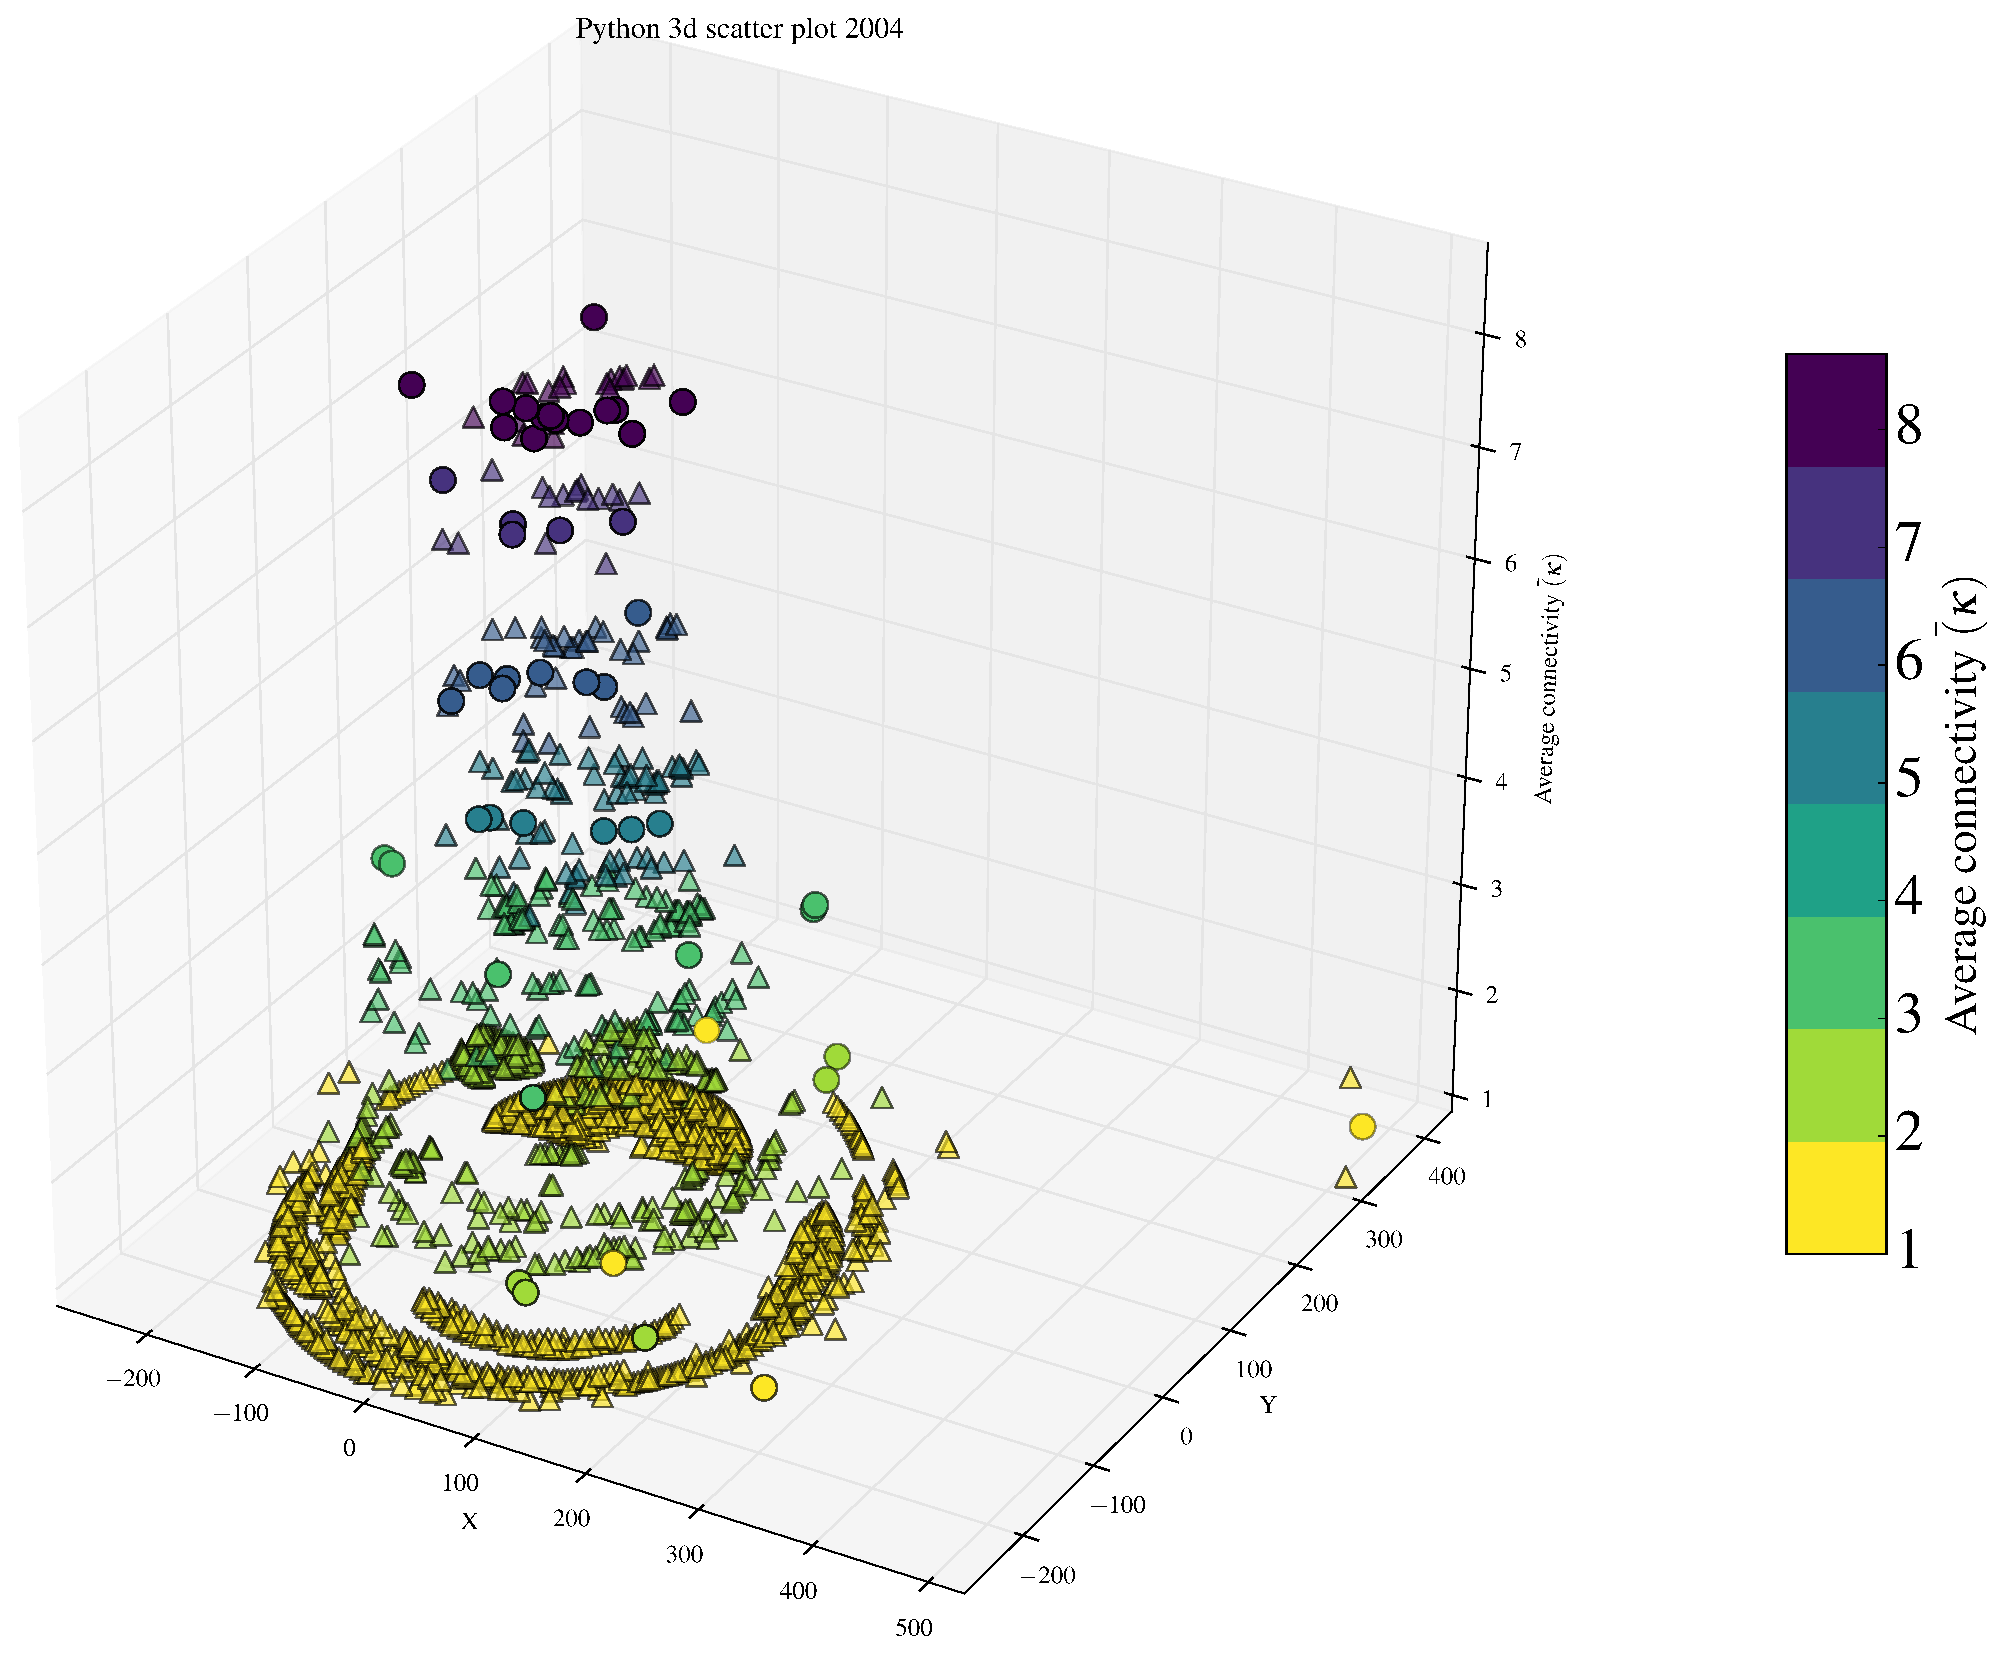
\includegraphics[scale=0.23]{figures/3d_scatter_python_2004}
}
\hspace{.01in}
\subfloat[Null model Python network 2004]{
\label{fig:s3d_null_python_2004}
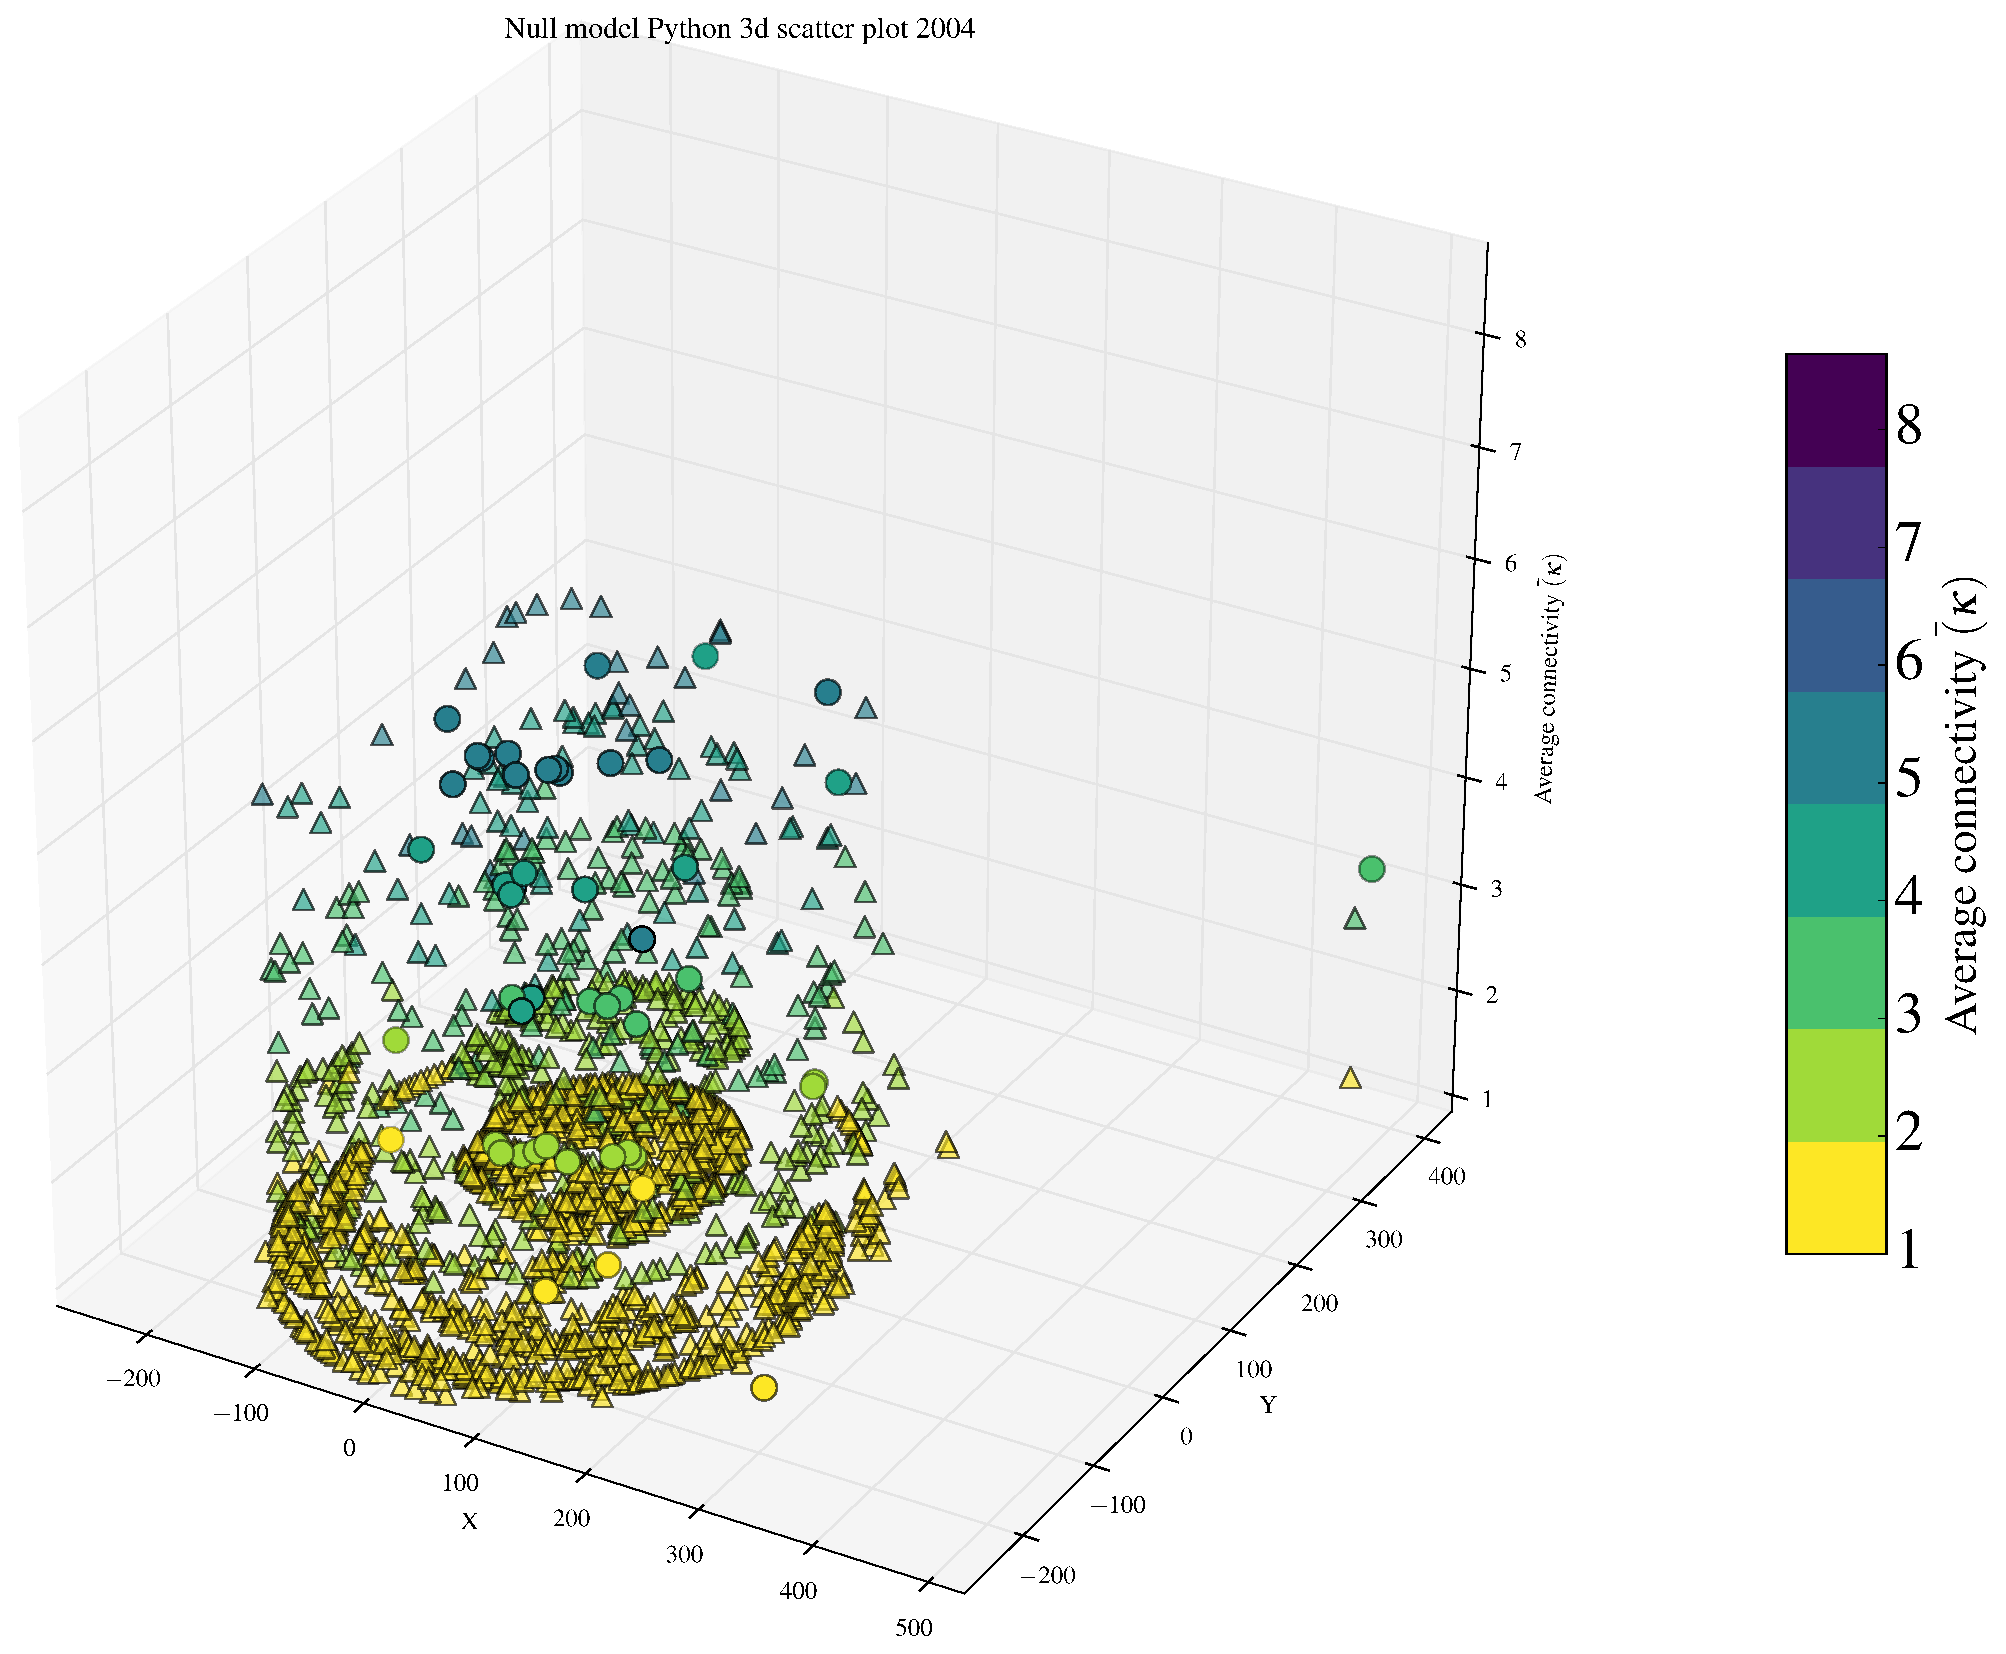
\includegraphics[scale=0.23]{figures/3d_scatter_python_2004_null}
}

\subfloat[Actual Python network 2013]{
\label{fig:s3d_actual_python_2013}
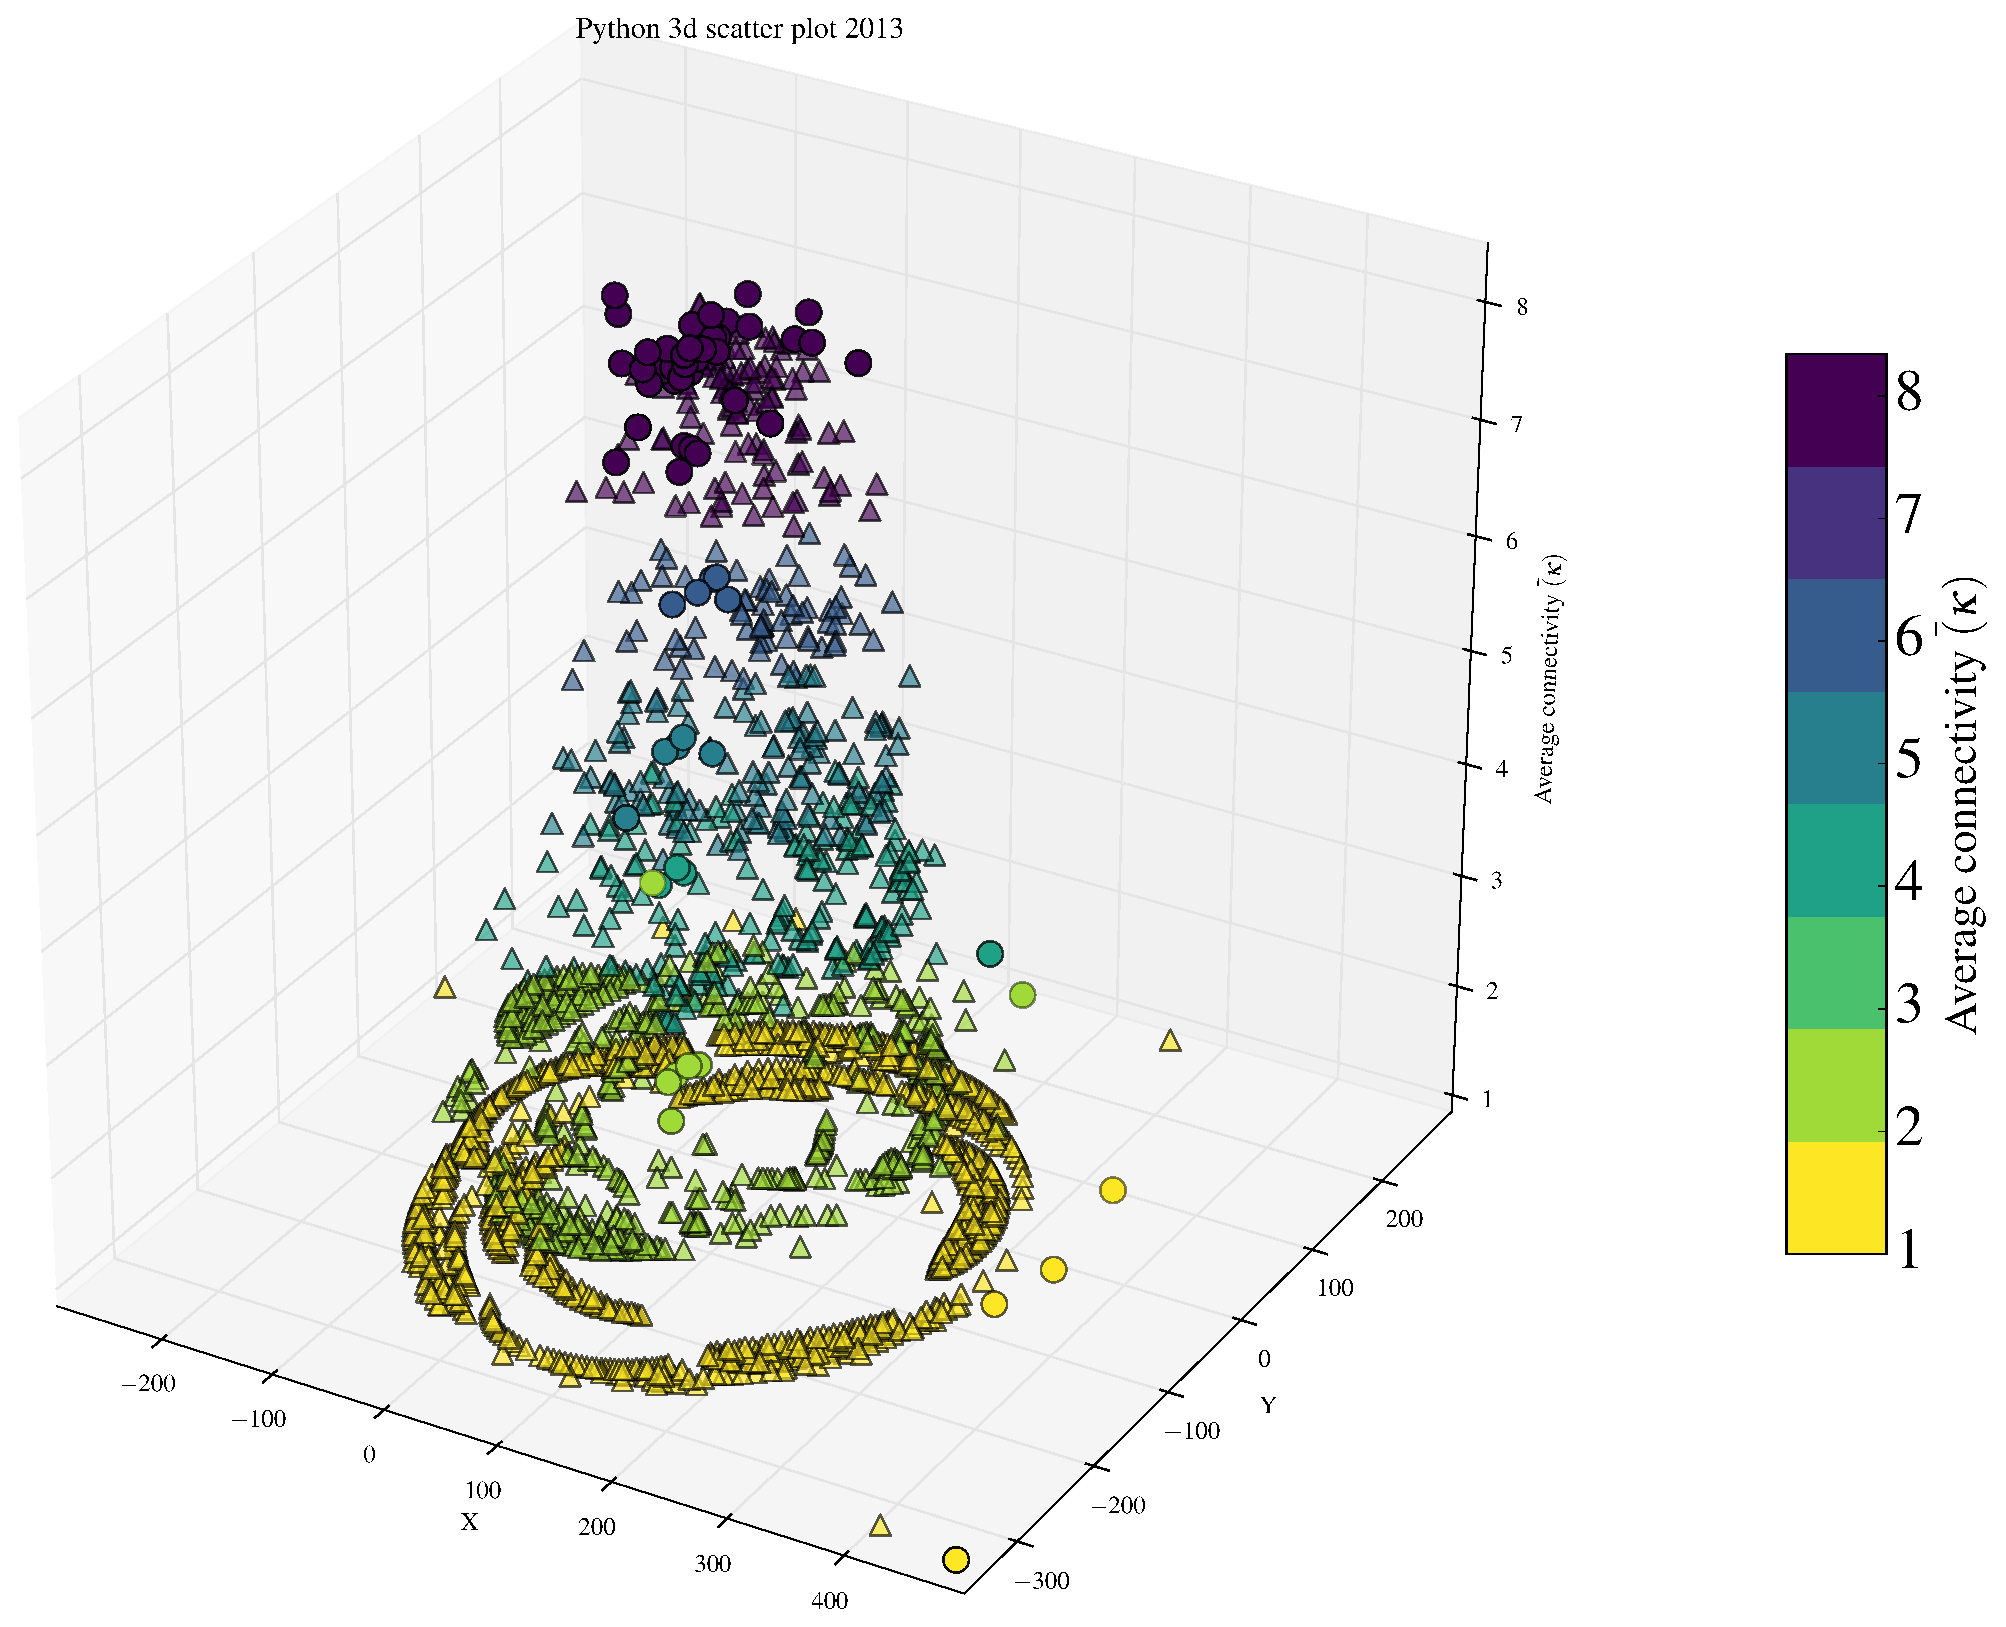
\includegraphics[scale=0.23]{figures/3d_scatter_python_2013}
}
\hspace{.01in}
\subfloat[Null model Python network 2013]{
\label{fig:s3d_null_python_2013}
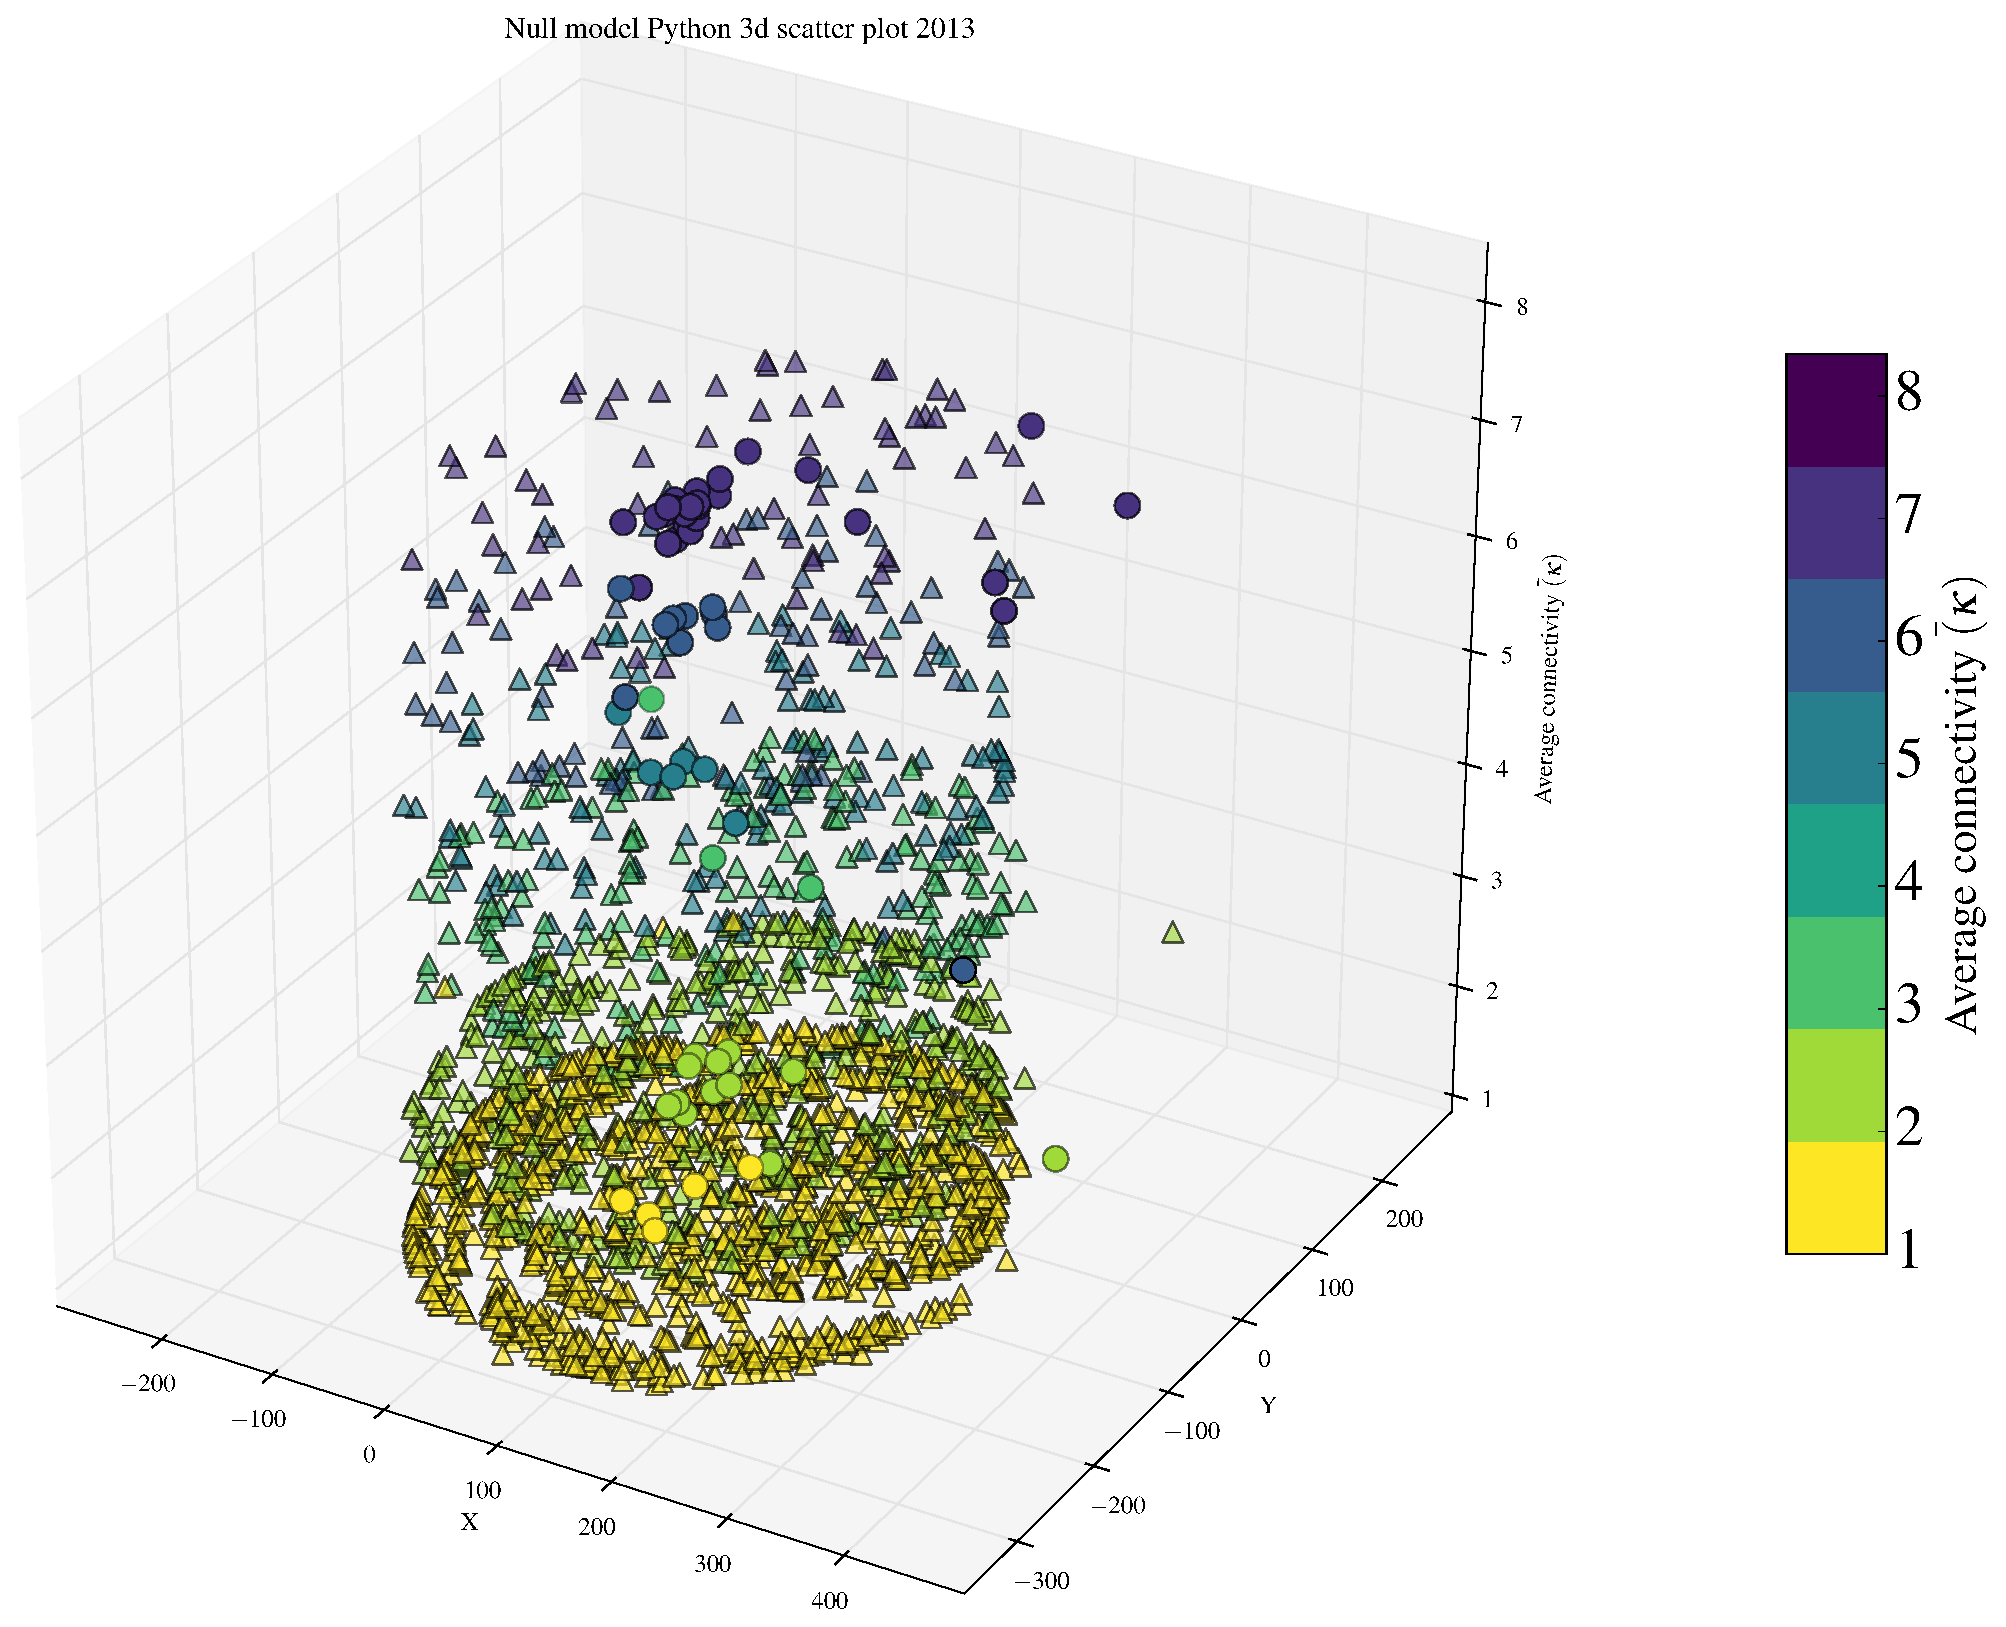
\includegraphics[scale=0.23]{figures/3d_scatter_python_2013_null}
}

\caption[Python average connectivity three-dimensional scatter plots.]{Python average connectivity three-dimensional scatter plots for actual networks and their random null models counterparts. X and Y are the positions determined by the Kamada-Kawai layout algorithm. The vertical dimension is average connectivity. Each mark is a node of the network as two-mode networks they contain both programs (triangles) and developers (circles).}
\label{fig:python-s3d}
\end{figure}


\begin{table}[H]
\begin{center}
\begin{tabular}{|c|c|c|c|c|c|c|c|}
\hline
Years&Nodes&GC&Random GC&GBC&Random GBC&maximum $k$&Random max $k$\\
\hline
1999&3,259&66.6\%&83.4\%&9.4\%&11.4\%&3 (0.2\%)&2 (11.4\%)\\
2000&3,593&52.5\%&77.8\%&7.0\%&10.7\%&3 (0.2\%)&2 (10.7\%)\\
2001&5,943&71.6\%&86.4\%&13.9\%&17.5\%&3 (0.1\%)&2 (17.5\%)\\
2002&6,857&72.4\%&88.1\%&12.7\%&17.0\%&4 (0.2\%)&2 (17.0\%)\\
2003&7,276&75.6\%&89.5\%&14.8\%&20.2\%&5 (0.2\%)&2 (20.2\%)\\
2004&7,984&78.4\%&94.4\%&22.1\%&27.7\%&5 (0.2\%)&2 (27.7\%)\\
2005&8,328&83.8\%&94.4\%&26.1\%&31.3\%&4 (0.5\%)&3 (4.5\%)\\
2006&9,599&84.2\%&96.7\%&33.7\%&39.0\%&4 (0.6\%)&3 (8.4\%)\\
2007&9,471&86.5\%&96.1\%&35.6\%&40.7\%&4 (0.2\%)&3 (8.6\%)\\
2008&10,662&87.2\%&96.4\%&34.3\%&40.3\%&4 (0.6\%)&3 (7.5\%)\\
2009&11,336&89.4\%&96.1\%&35.7\%&42.3\%&5 (0.4\%)&3 (8.2\%)\\
2010&10,515&86.9\%&95.5\%&32.7\%&39.8\%&5 (0.2\%)&3 (5.1\%)\\
2011&12,362&87.7\%&95.0\%&30.6\%&36.0\%&5 (0.3\%)&3 (5.3\%)\\
2012&11,904&87.1\%&95.0\%&31.0\%&36.7\%&4 (0.1\%)&3 (2.3\%)\\
\hline
\end{tabular}
\caption{Structural Cohesion metrics for debian networks.}
\label{str_cohesion_debian}
\end{center}
\end{table}




\begin{figure}[p]
%\centering
\subfloat[Actual Debian network 2000]{
\label{fig:s3d_actual_debian_2000}
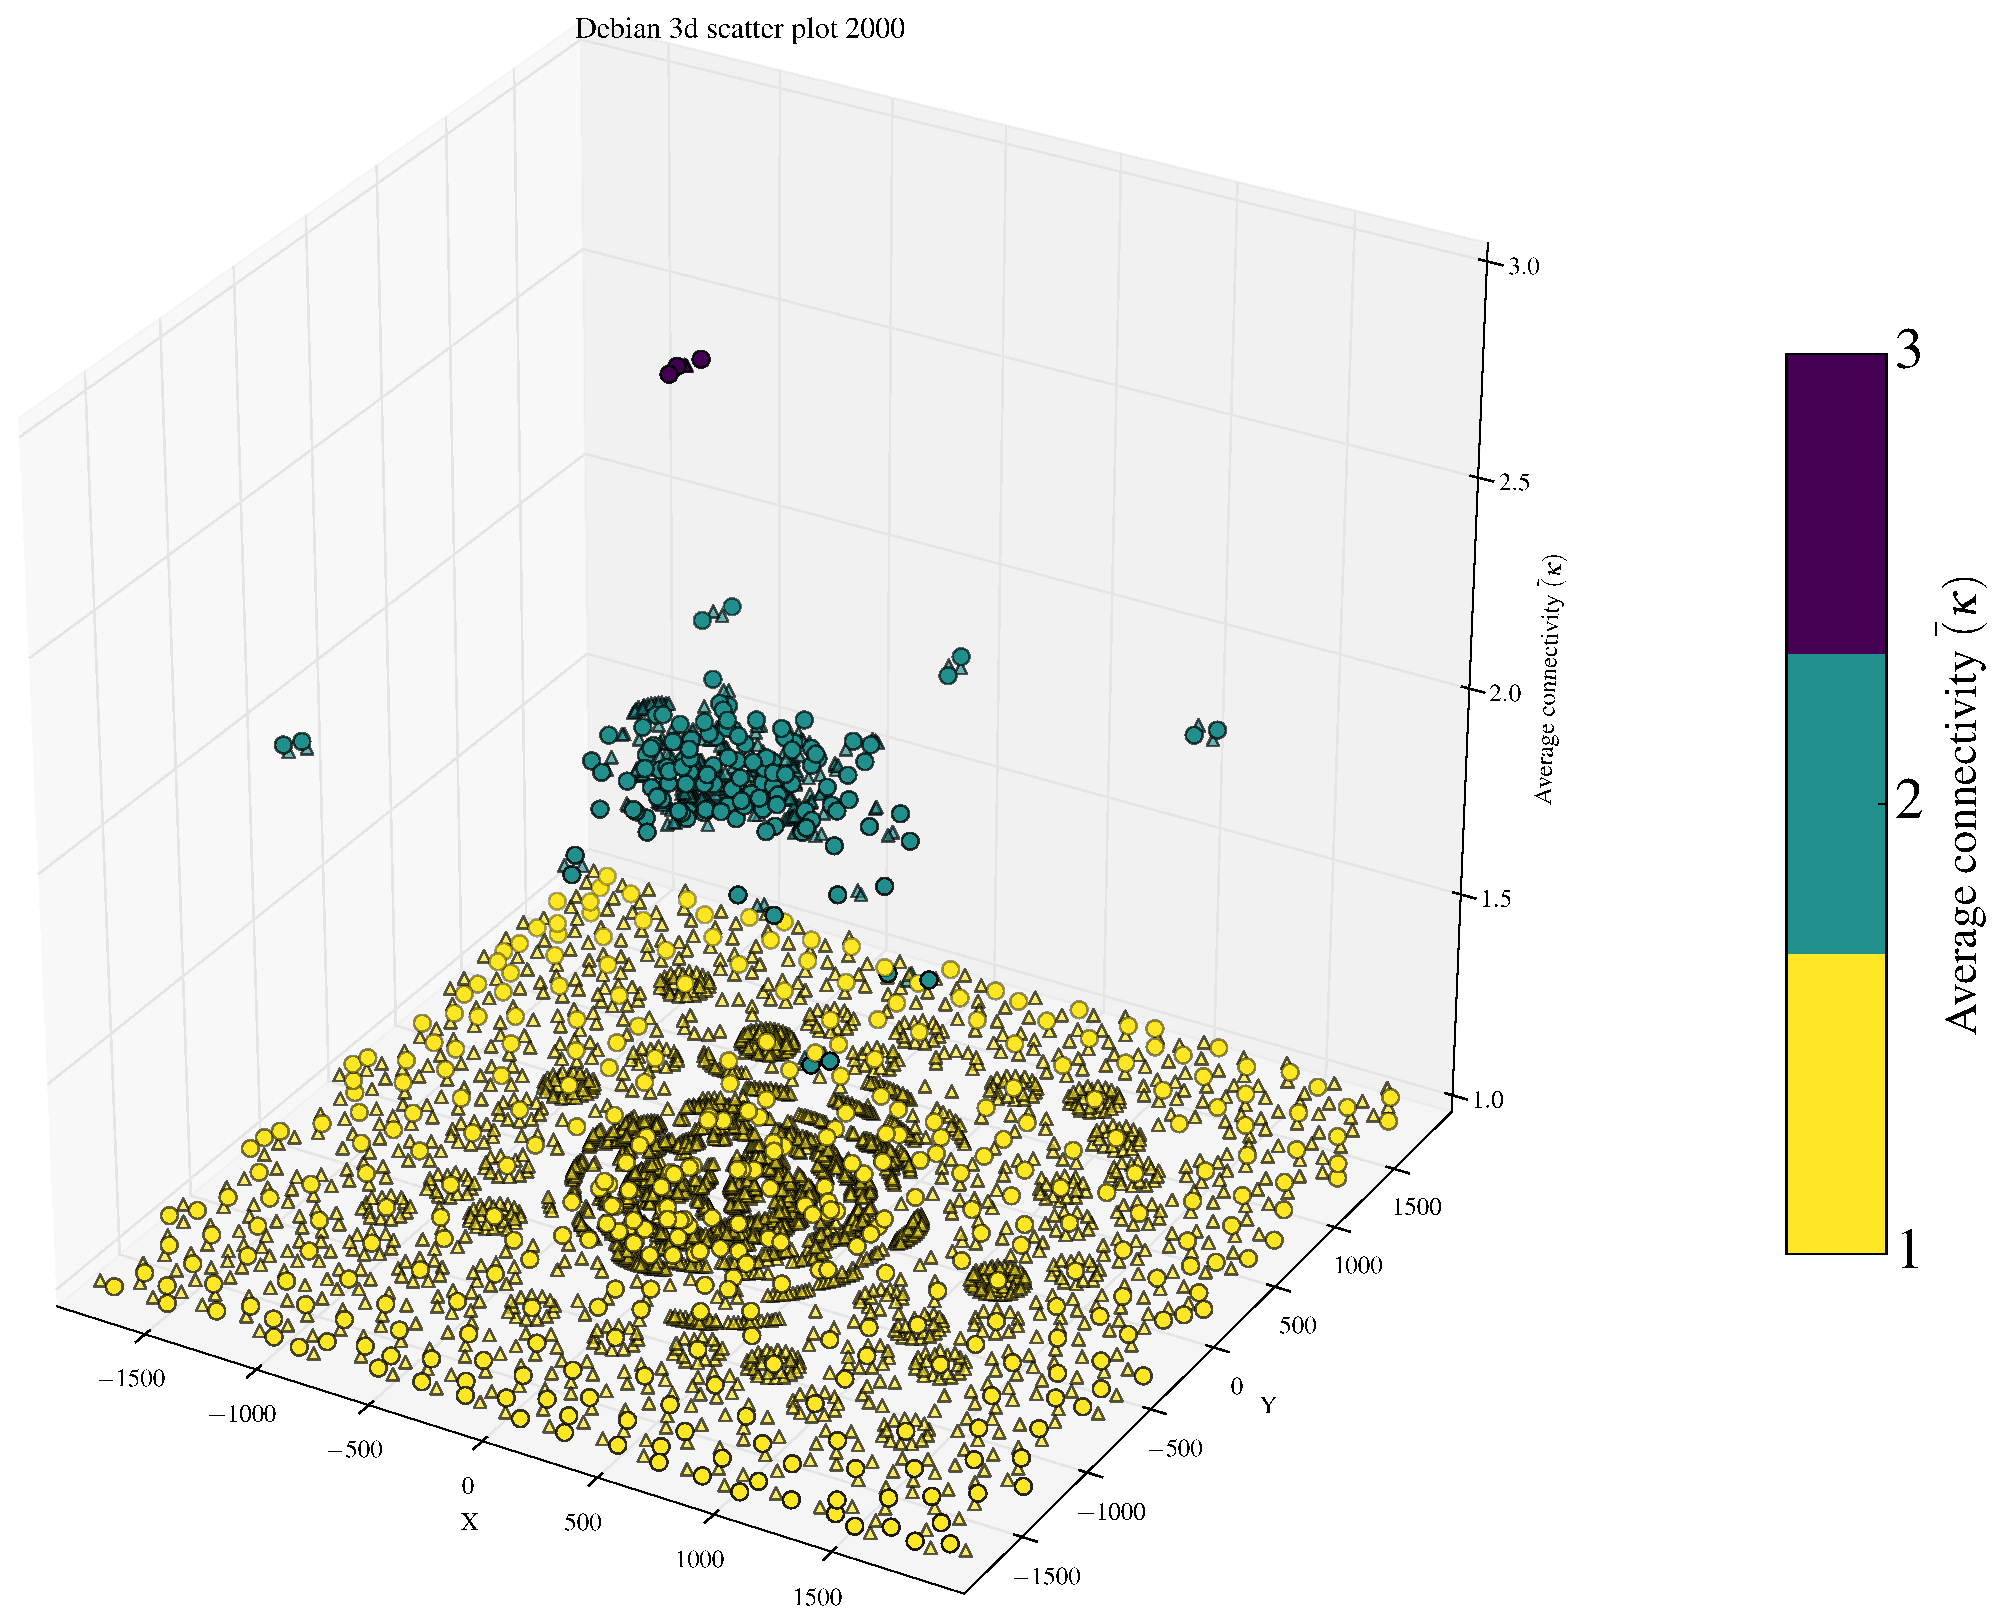
\includegraphics[scale=0.23]{figures/3d_scatter_debian_2000}
}
\hspace{.01in}
\subfloat[Null model Debian network 2000]{
\label{fig:s3d_null_debian_2000}
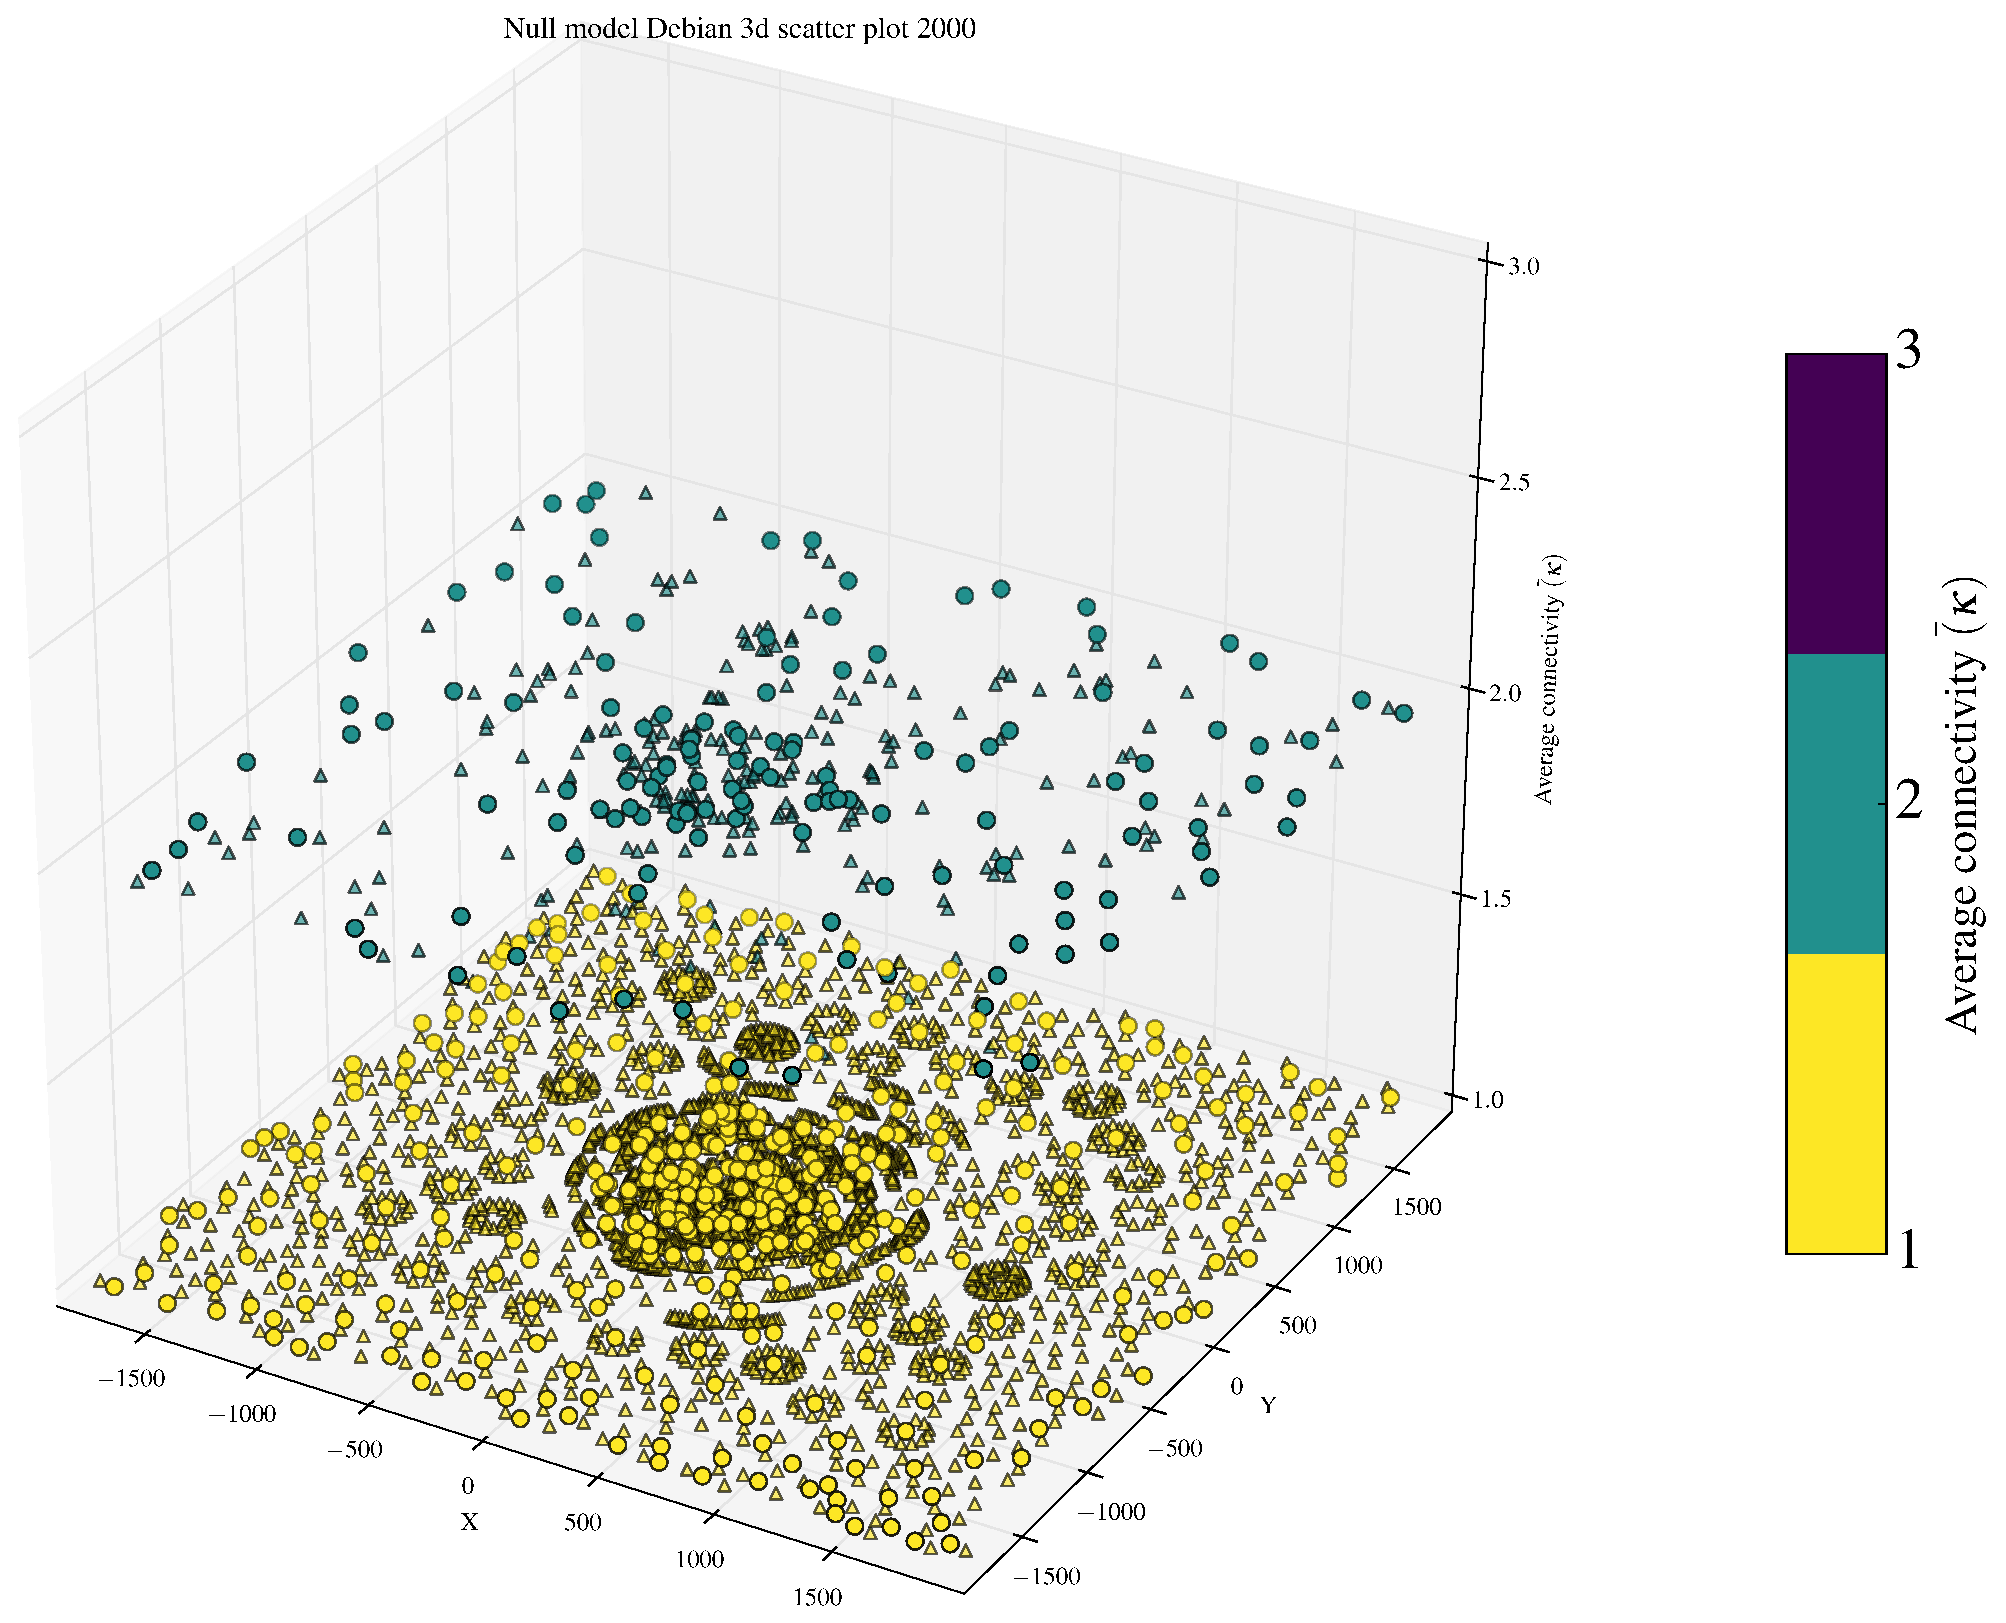
\includegraphics[scale=0.23]{figures/3d_scatter_debian_2000_null}
}

\subfloat[Actual Debian network 2004]{
\label{fig:s3d_actual_debian_2004}
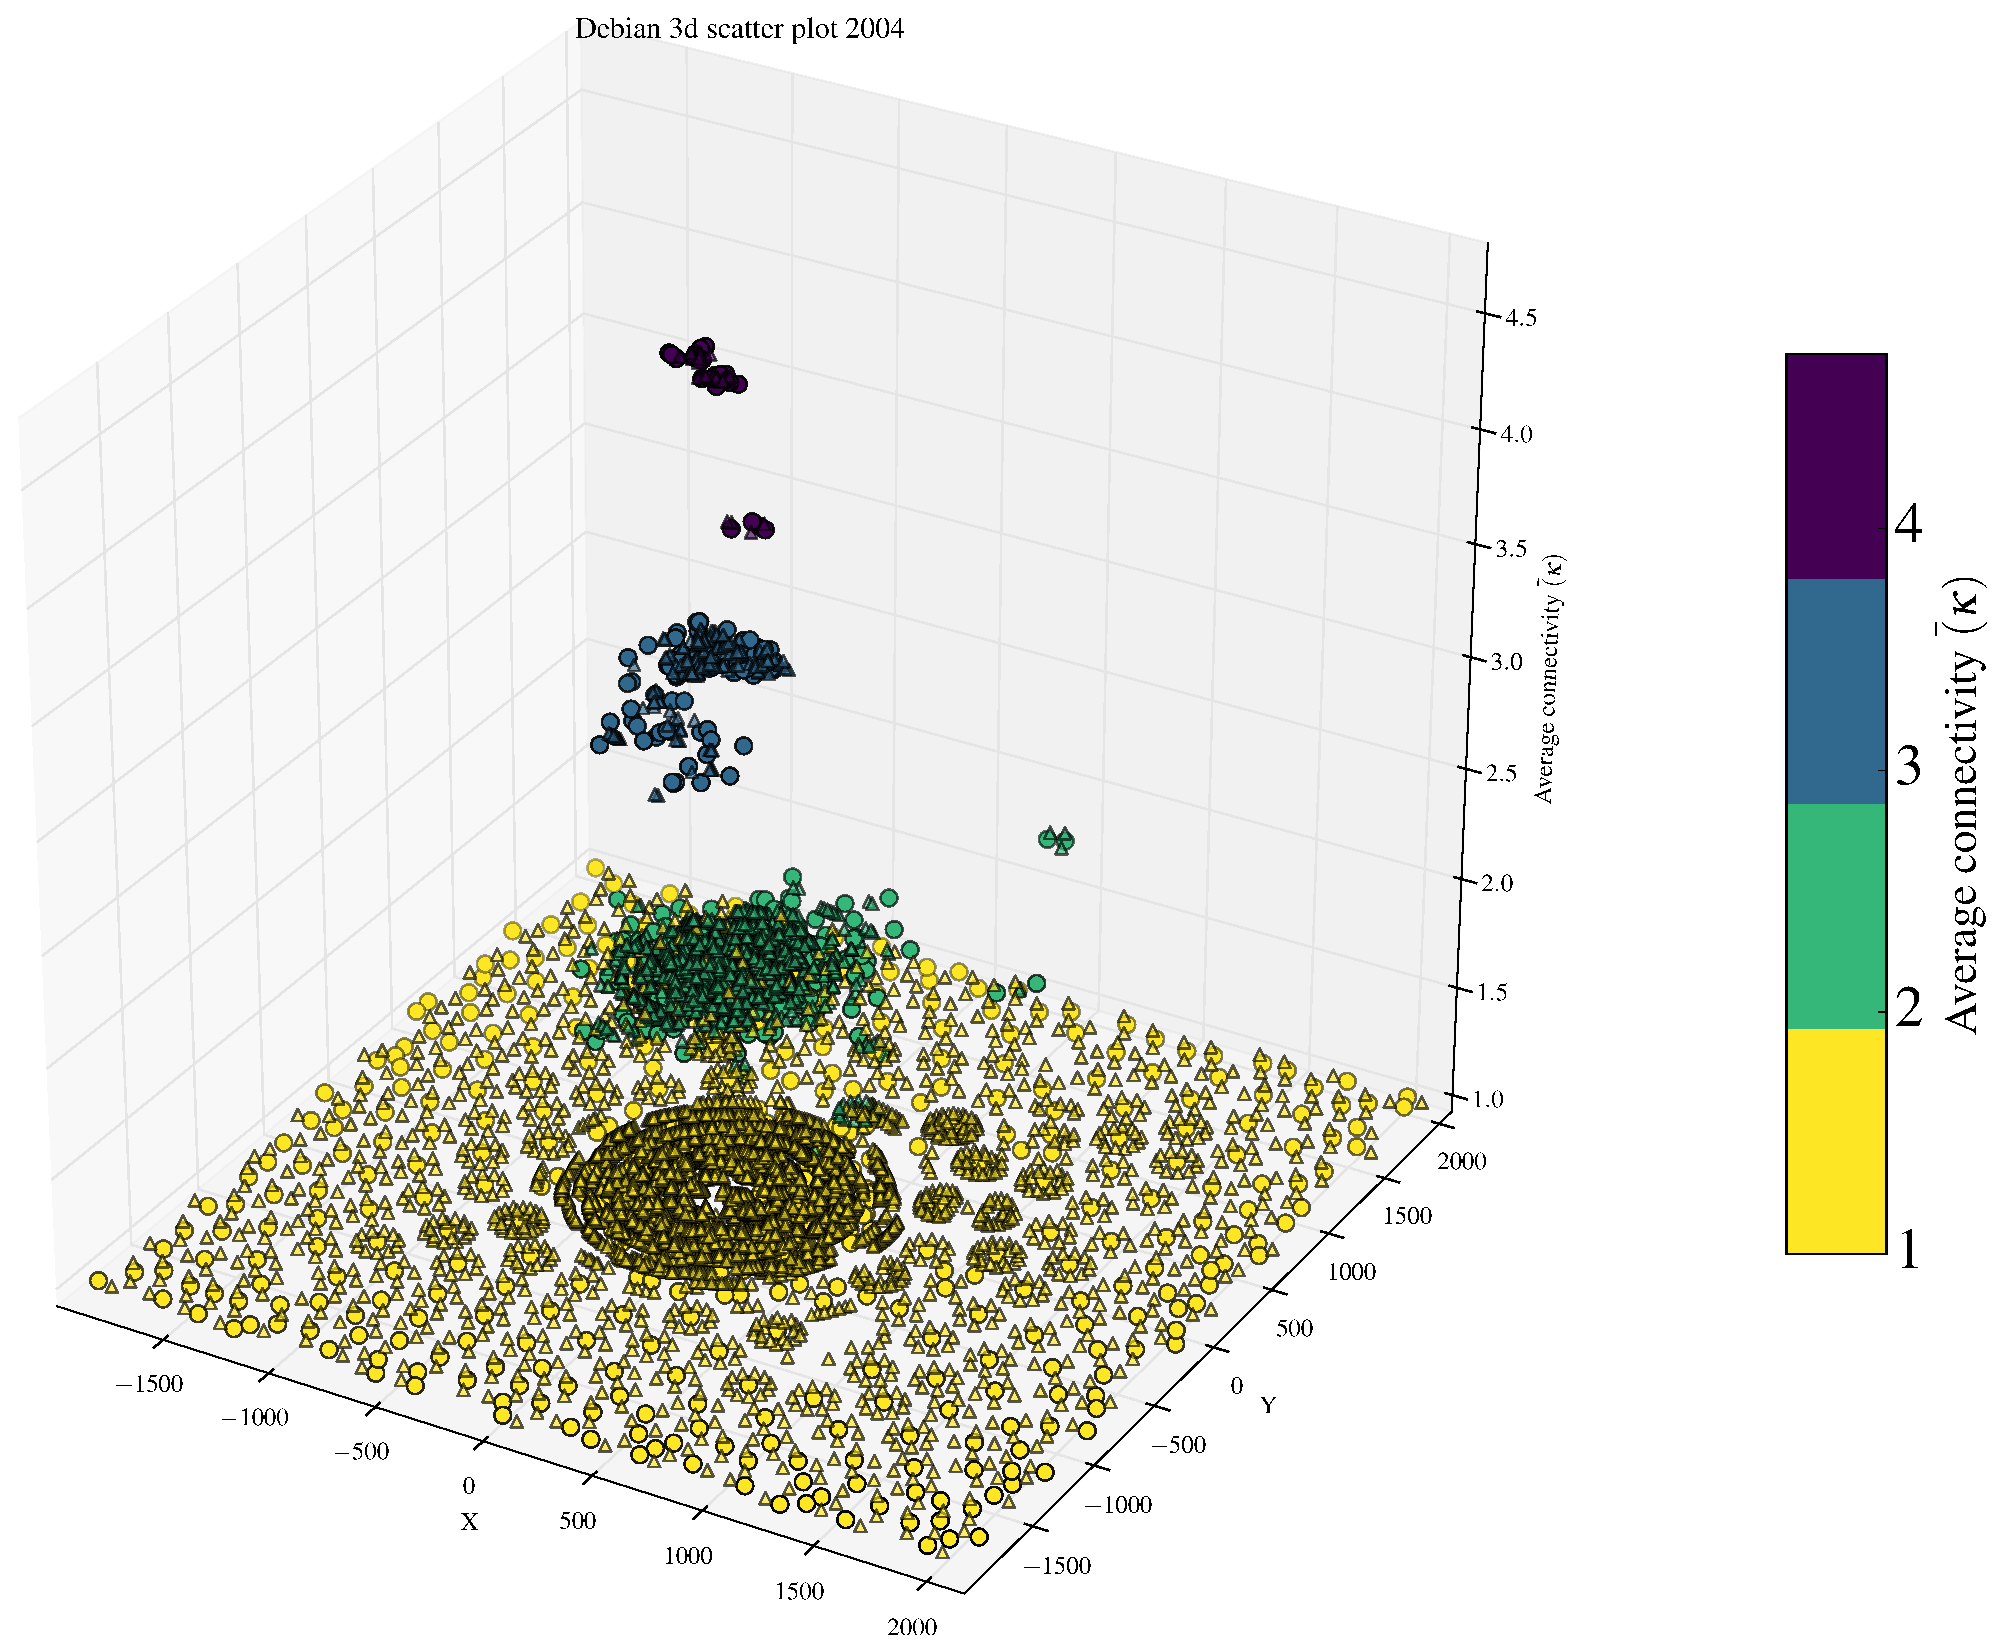
\includegraphics[scale=0.23]{figures/3d_scatter_debian_2004}
}
\hspace{.01in}
\subfloat[Null model Debian network 2004]{
\label{fig:s3d_null_debian_2004}
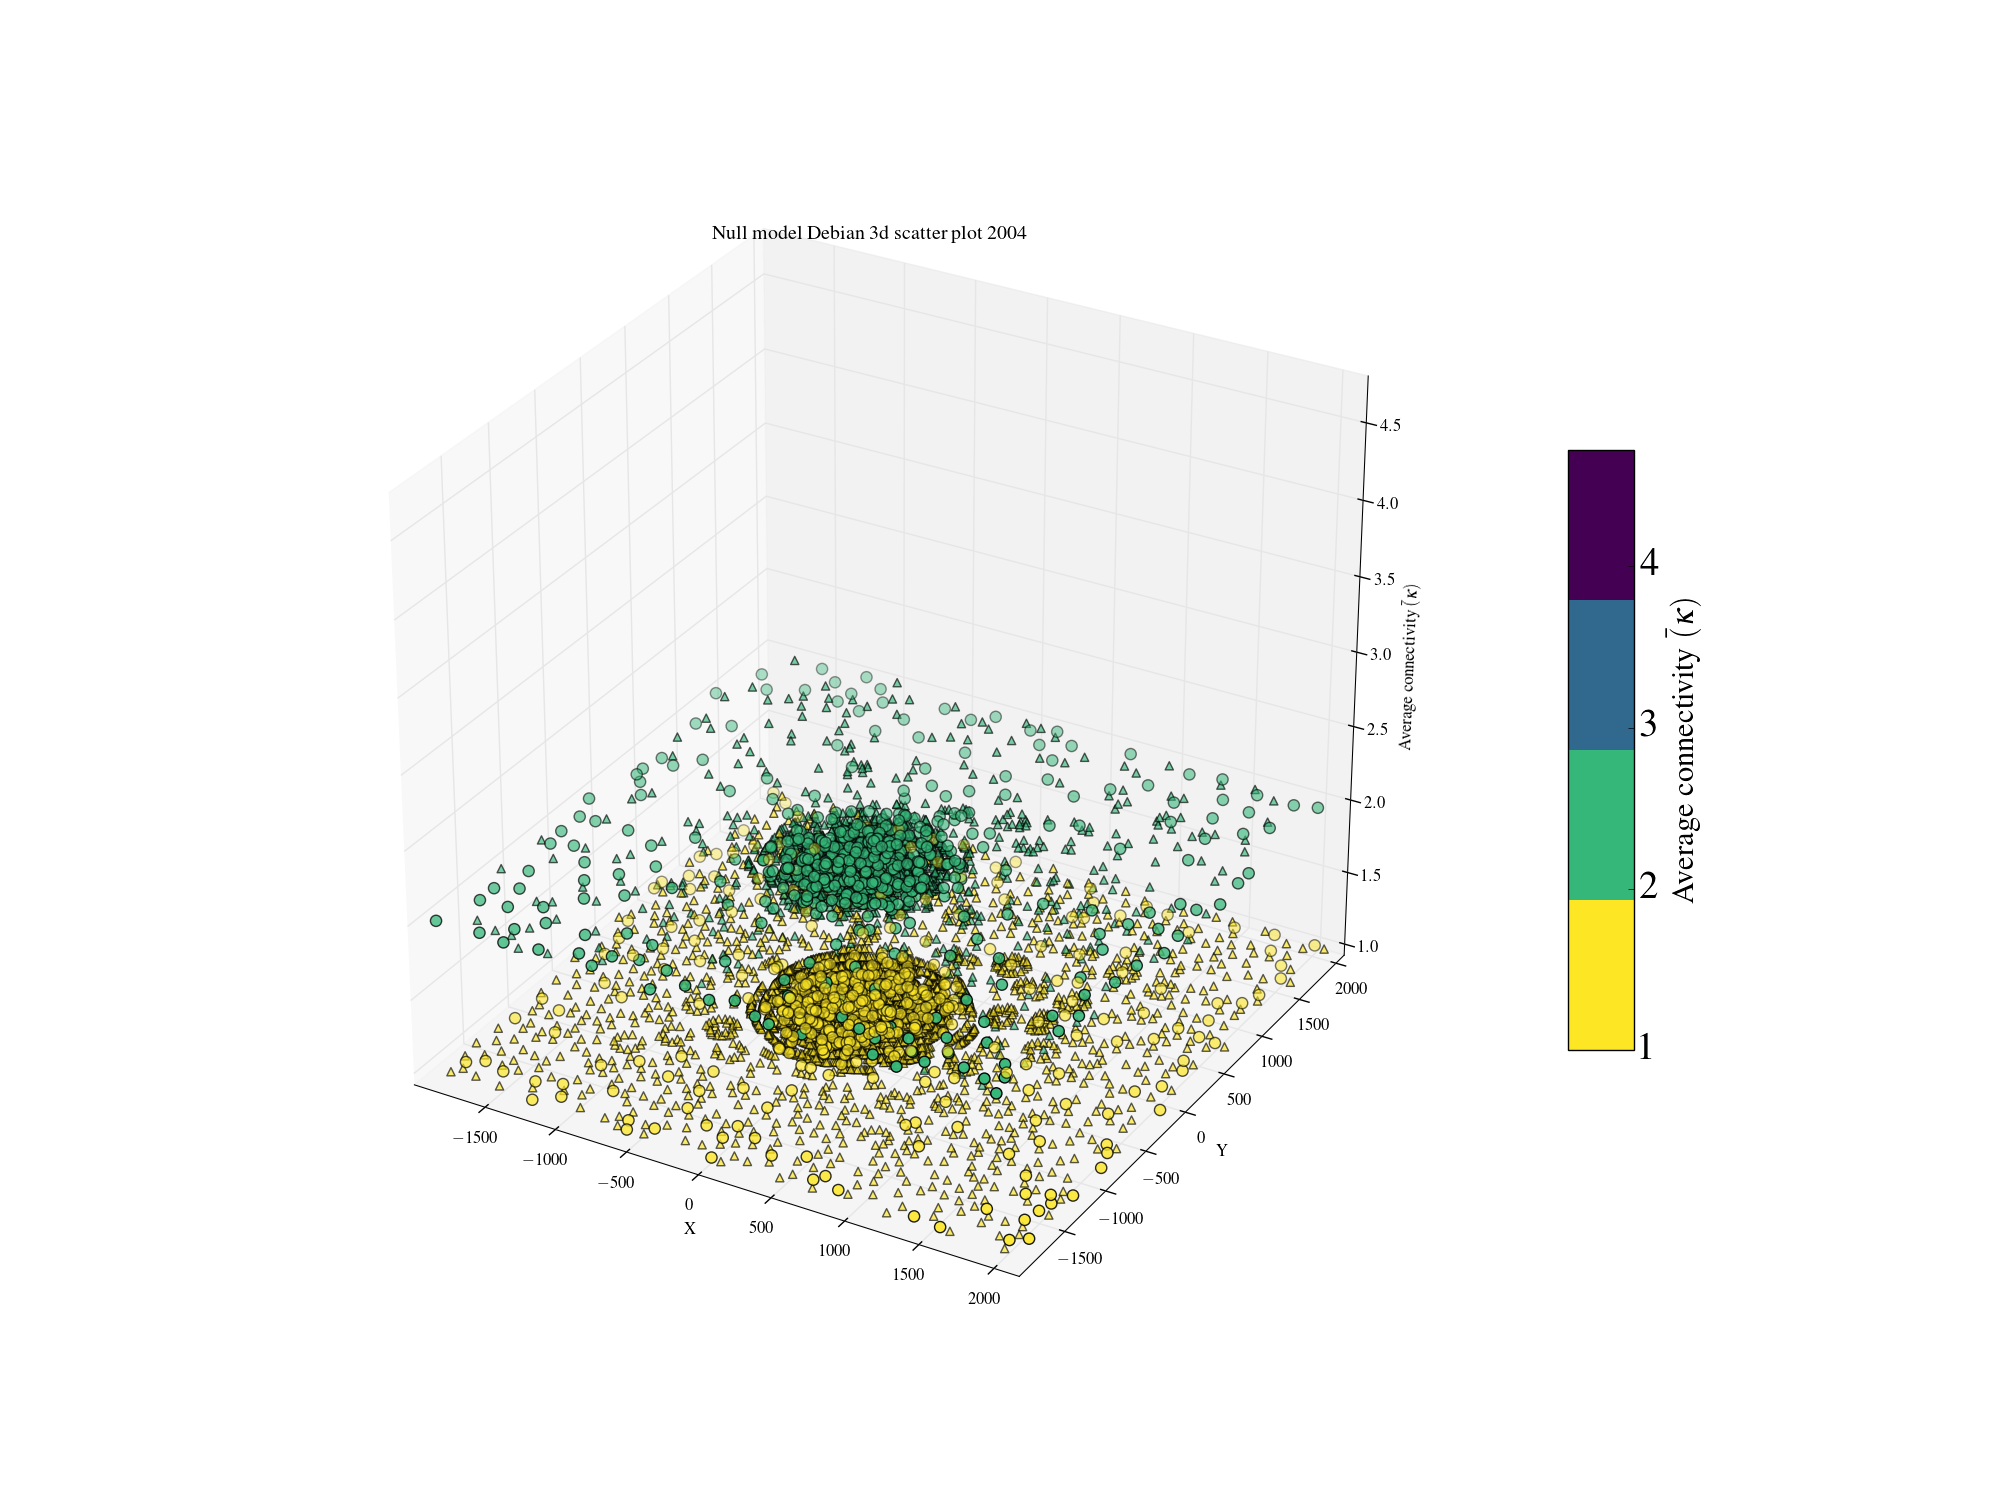
\includegraphics[scale=0.23]{figures/3d_scatter_debian_2004_null}
}

\subfloat[Actual Debian network 2011]{
\label{fig:s3d_actual_debian_2011}
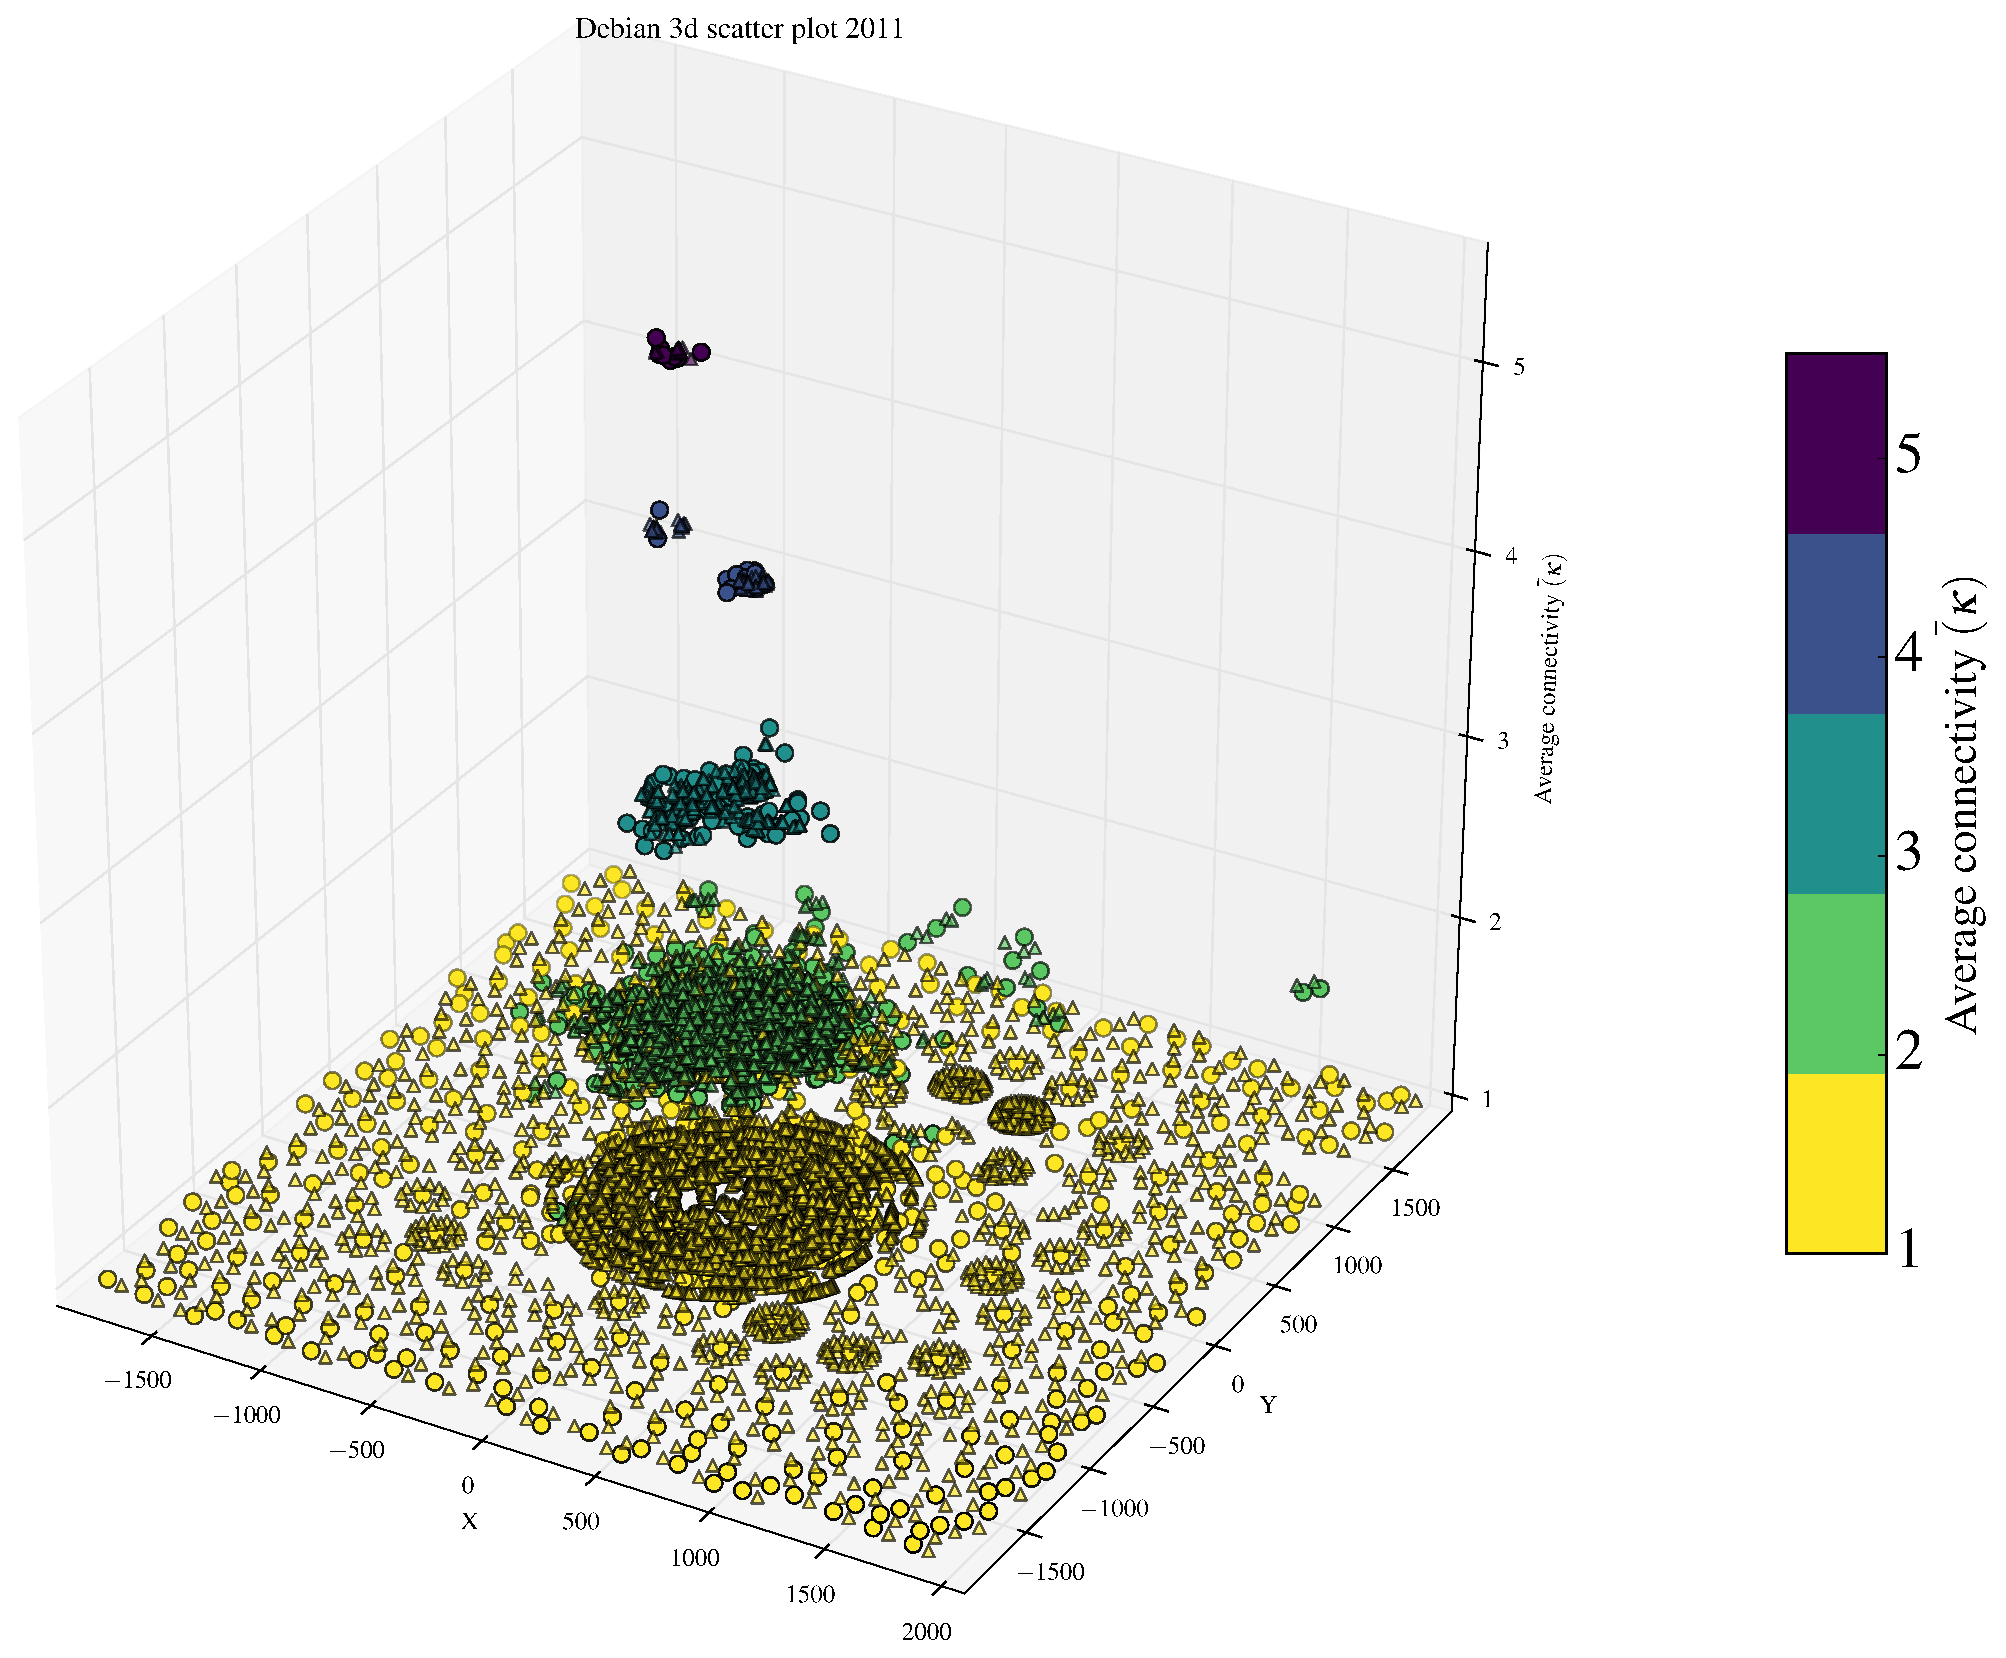
\includegraphics[scale=0.23]{figures/3d_scatter_debian_2011}
}
\hspace{.01in}
\subfloat[Null model Debian network 2011]{
\label{fig:s3d_null_debian_2011}
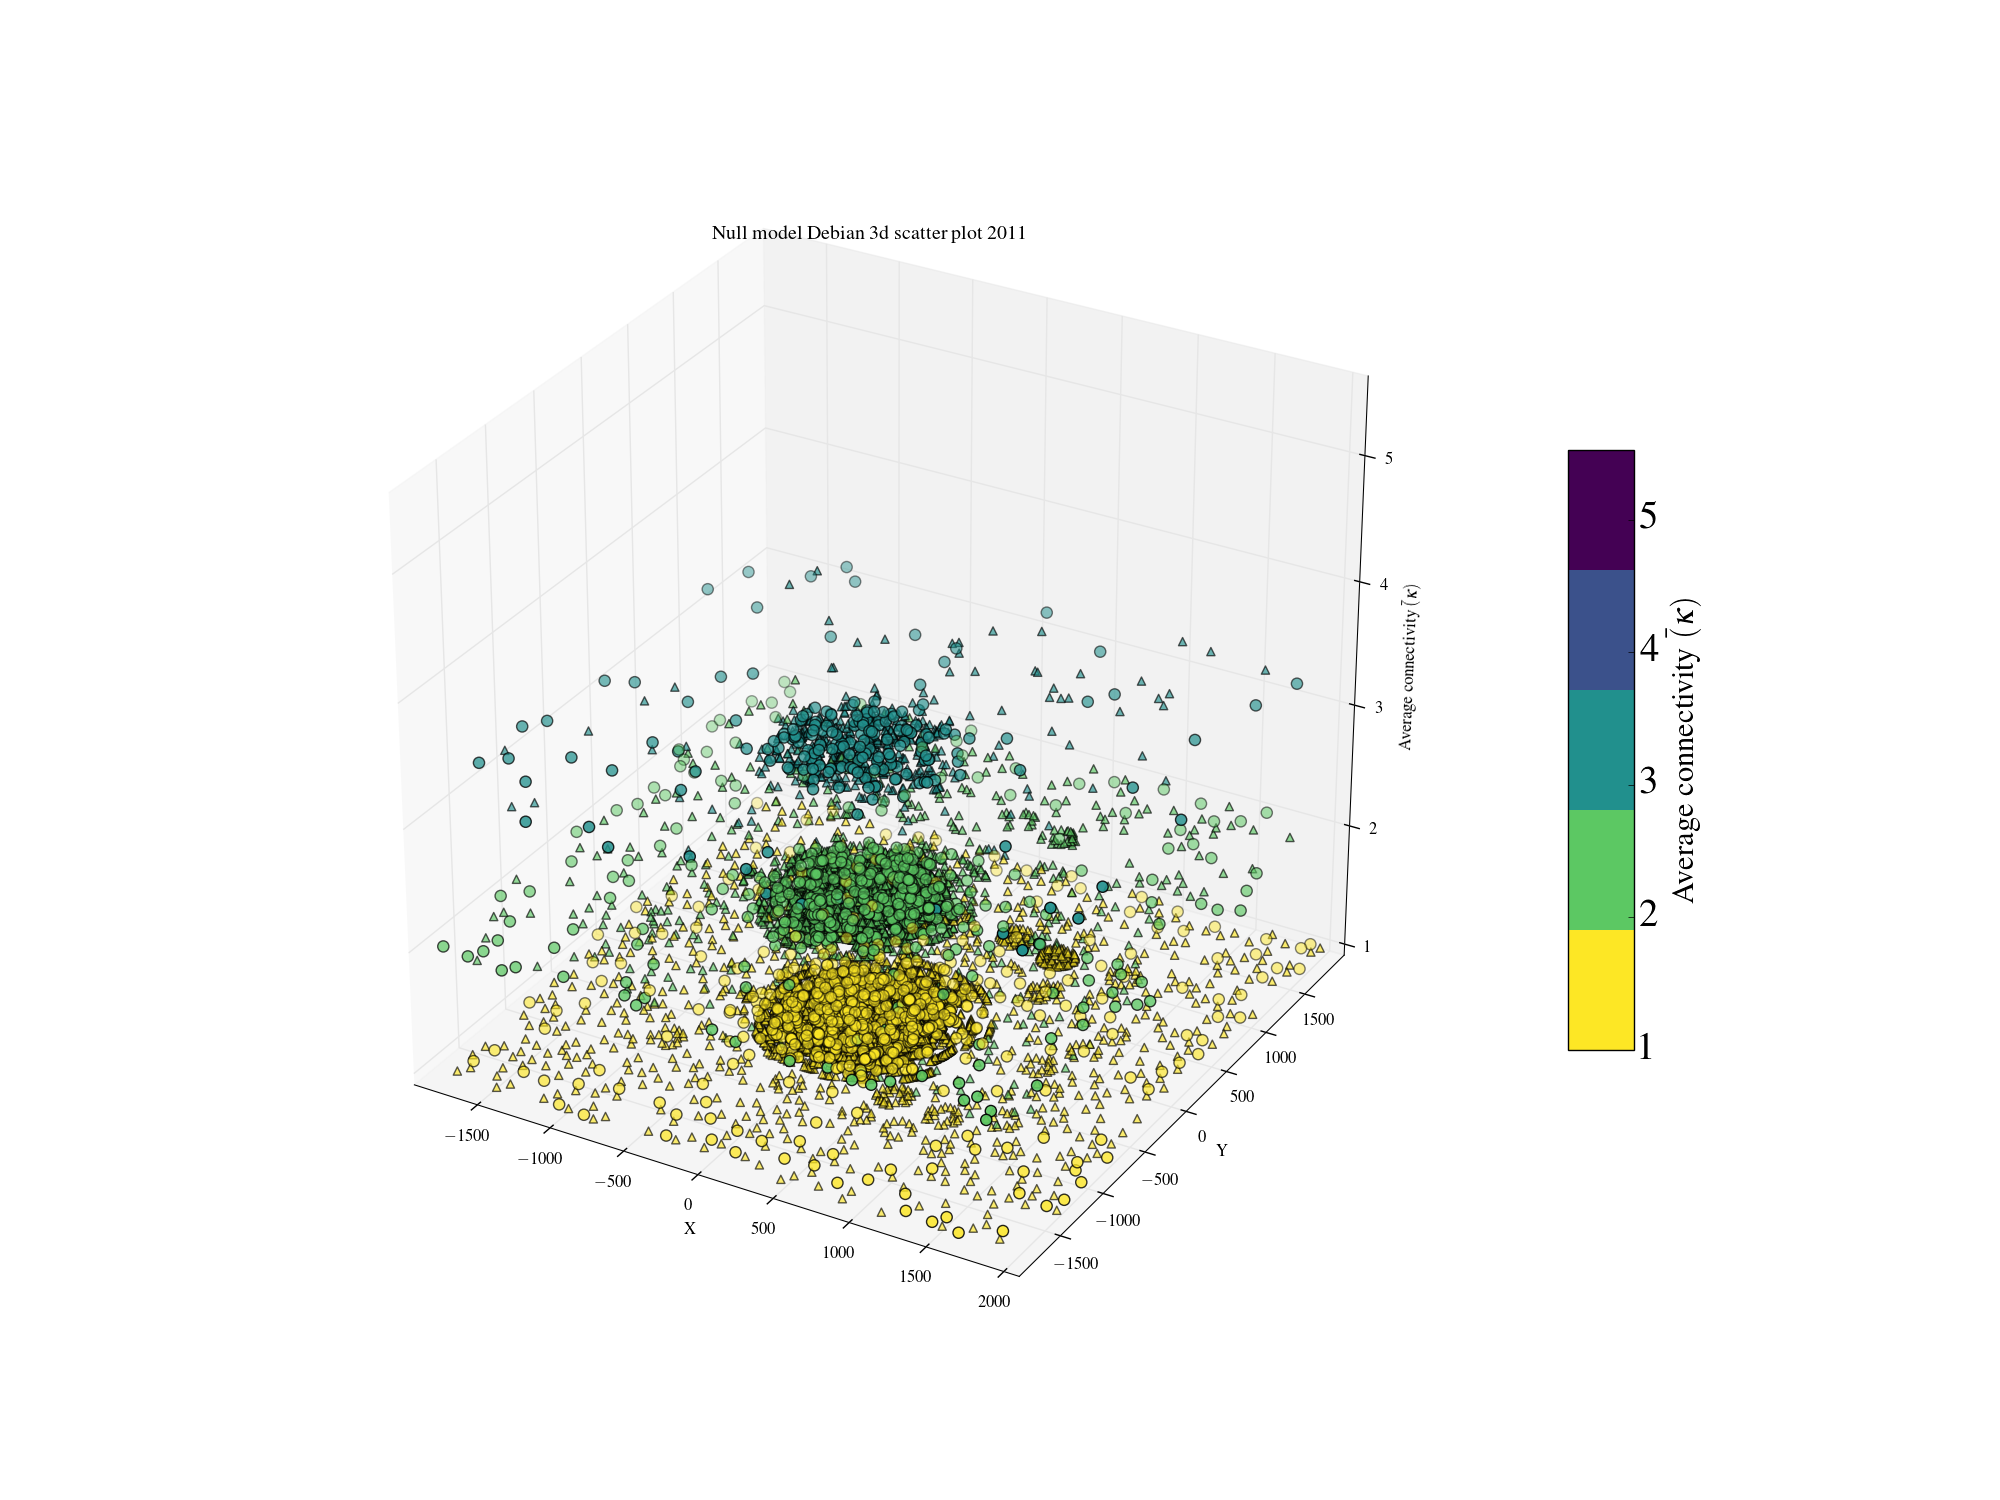
\includegraphics[scale=0.23]{figures/3d_scatter_debian_2011_null}
}

\caption[Debian average connectivity three-dimensional scatter plots.]{Debian average connectivity three-dimensional scatter plots for actual networks and their random null models counterparts. X and Y are the positions determined by the Kamada-Kawai layout algorithm. The vertical dimension is average connectivity. Each mark is a node of the network as two-mode networks they contain both programs (triangles) and developers (circles).}
\label{fig:debian-s3d}
\end{figure}

